\chapter{Operation Model}
\label{chap:lu.uni.lassy.excalibur.examples.icrash-OM}

This section contains the operation schemes of each operation defined in either an actor, its output interface, in a primary or secondary type (class, datatype or enumeration types). 
The \msrmessir OCL code listing is joined to the comment table.

\lstset{
float,
basicstyle=\scriptsize,
language=Messir,
breakatwhitespace=false,
tabsize=2,
breaklines=true,
numbers=left,
emptylines=1,
numbersep=5pt,
showspaces=false,
showstringspaces=false,
showtabs=false
} 


%% ***************************************************************
%% operations for: Environment-Out Interface Operation Schemes

		
\section{Environment - Out Interface Operation Scheme for actActivator}
\label{OM-EM-OutInterface-OS-actActivator}
\subsection{Operation Model for oeSetClock}

\label{OM-oeSetClock}


The \msrcode{oeSetClock} operation has the following properties:

	\begin{operationmodel}
	\addheading{Operation}
	\adddoublerow{oeSetClock[proactive]}{ 
	An active message used to statically set the date and time information in the system's state. 
	}

	\addrowheading{Parameters}
	\addnumbereddoublerow{}{AcurrentClock: dtDateAndTime}{ the date and time to be considered as the actual one.} 

	\addrowheading{Return type}
	\addsinglerow{ptBoolean}

	\addrowheading{Pre-Condition (protocol)}
	\addnumberedsinglerow{PreP}{ the system is supposed to be created and initialized and the provided date and time value is greater than the one known by the system.}
		
	\addrowheading{Pre-Condition (functional)}
	\addnumberedsinglerow{PreF}{ none }

	\addrowheading{Post-Condition (functional)}
	\addnumberedsinglerow{PostF}{ 
	the ctState instance post-state is updated to have its clock attribute equal to the given date and time.
	}

	\addrowheading{Post-Condition (protocol)}
	\addnumberedsinglerow{PostP}{none}
	\end{operationmodel}



	% ------------------------------------------
	% MCL Listing
	% ------------------------------------------
	\vspace{1cm}
	The listing~\ref{OM-actActivator-oeSetClock-MCL-LST} provides the \msrmessir (MCL-oriented) specification of the operation.
	
	\scriptsize
	\vspace{0.5cm}
	\begin{lstlisting}[style=MessirStyle,firstnumber=auto,captionpos=b,caption={\msrmessir (MCL-oriented) specification of the operation \emph{oeSetClock}.},label=OM-actActivator-oeSetClock-MCL-LST]

	/* Pre Protocol:*/ 
	preP{let TheSystem: ctState in
	  let AvpStarted: ptBoolean in
	  
	/* PreP01 */
	  self.rnActor.rnSystem = TheSystem
	  and self.rnActor.rnSystem.vpStarted = AvpStarted
	  and AvpStarted = true
	  and TheSystem.clock.lt(AcurrentClock)}
	
	/* Pre Functional:*/
	preF{true}
	
	/* Post Functional:*/ 
	postF{let TheSystem: ctState in
	  self.rnActor.rnSystem = TheSystem
	
	/* PostF01 */
	  and TheSystem@post.clock = AcurrentClock}
	
	/* Post Protocol:*/ 
	postP{ true}
	
	\end{lstlisting}
	\normalsize 
	
	
	
	






\subsection{Operation Model for oeSollicitateCrisisHandling}

\label{OM-oeSollicitateCrisisHandling}


The \msrcode{oeSollicitateCrisisHandling} operation has the following properties:

	\begin{operationmodel}
	\addheading{Operation}
	\adddoublerow{oeSollicitateCrisisHandling[proactive]}{A proactive message (message of a pro-active actor with no parameter triggered automatically if the pre protocol condition is true) used to avoid crisis to stay too long in an not handled status.}


	\addrowheading{Return type}
	\addsinglerow{ptBoolean}

	\addrowheading{Pre-Condition (protocol)}
	\addnumberedsinglerow{PreP}{the system is started}
	\addnumberedsinglerow{PreP}{ there exist some crisis that are in pending status and for which the duration between the current ctState clock information and the last reminder is greater than the crisis reminder period duration.}
		
	\addrowheading{Pre-Condition (functional)}
	\addnumberedsinglerow{PreF}{none}

	\addrowheading{Post-Condition (functional)}
	\addnumberedsinglerow{PostF}{if there exist coordinators and crisis who stood in a not handled status more than the maximum allowed time 
	then those crisis are randomly allocated to the existing coordinators.}
	\addnumberedsinglerow{PostF}{for all other crisis who stood too longly in a not handled status but not more than the maximum delay allowed 
	then a reminder message is sent to the administrator and all coordinator actors of the environment to sollicitate handling of those crisis.}

	\addrowheading{Post-Condition (protocol)}
	\addnumberedsinglerow{PostP}{the value of the last reminder known by the system at post state is the system's clock value.}
	\end{operationmodel}



	% ------------------------------------------
	% MCL Listing
	% ------------------------------------------
	\vspace{1cm}
	The listing~\ref{OM-actActivator-oeSollicitateCrisisHandling-MCL-LST} provides the \msrmessir (MCL-oriented) specification of the operation.
	
	\scriptsize
	\vspace{0.5cm}
	\begin{lstlisting}[style=MessirStyle,firstnumber=auto,captionpos=b,caption={\msrmessir (MCL-oriented) specification of the operation \emph{oeSollicitateCrisisHandling}.},label=OM-actActivator-oeSollicitateCrisisHandling-MCL-LST]

	/* Pre Protocol:*/ 
	preP{let TheSystem: ctState in
	  let AvpStarted: ptBoolean in
	  let ColctCrisisToHandle:
	        Bag(ctCrisis) in
	  
	  self.rnActor.rnSystem = TheSystem
	    
	/* PreP01 */
	  and TheSystem.vpStarted
	  
	/* PreP02 */
	  and TheSystem.rnctCrisis->select(handlingDelayPassed()) 
	      = ColctCrisisToHandle
	  and ColctCrisisToHandle->size().geq(1)}
	
	/* Pre Functional:*/
	preF{true}
	
	/* Post Functional:*/ 
	postF{let TheSystem: ctState in
	  let AMessageForCrisisHandlers: dtComment in
	  let ColctCrisisToAllocateIfPossible:Bag(ctCrisis) in
	  
	  self.rnActor.rnSystem = TheSystem
	/* PostF01 */
	  and TheSystem.rnctCrisis->select(maxHandlingDelayPassed())
	      = ColctCrisisToAllocateIfPossible
	  and  ColctCrisisToAllocateIfPossible->forAll(isAllocatedIfPossible())
	
	 /* PostF02 */
	  and TheSystem.rnctCrisis->select(handlingDelayPassed())
	  = ColctCrisisToHandle
	  
	  and ColctCrisisToHandle->msrColSubtract(ColctCrisisToAllocateIfPossible)
	      = ColctCrisisToRemind
	      
	  and if (ColctCrisisToRemind->size().geq(1))
	      then (AMessageForCrisisHandlers.value
	            ='There are alerts pending since more than the defined delay. Please REACT !'
	            and TheSystem.rnactAdministrator.
	                rnInterfaceIN^ieMessage(AMessageForCrisisHandlers)
	                and TheSystem.rnactCoordinator
	                    ->forAll(rnInterfaceIN^ieMessage(AMessageForCrisisHandlers))
	            )
	      else true
	      endif}
	
	/* Post Protocol:*/ 
	postP{ let TheSystem: ctState in
	  let TheClock: dtDateAndTime in
	  
	  self.rnActor.rnSystem = TheSystem
	  and TheSystem.clock = TheClock
	  and TheSystem@post.vpLastReminder = TheClock}
	
	\end{lstlisting}
	\normalsize 
	
	
	
	





Figure \ref{fig:lu.uni.lassy.excalibur.examples.icrash-OM-scopeView-operation-scope-outactActivator-oeSollicitateCrisisHandling}
shows concept model elements in the scope of the oeSollicitateCrisisHandling operation

\begin{figure}[htbp]
\begin{center}

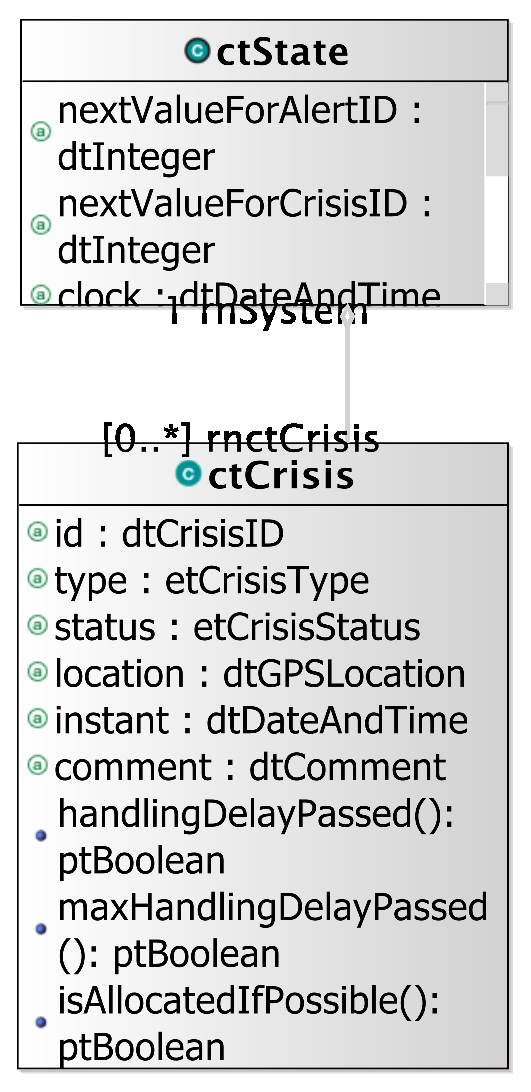
\includegraphics[
angle=0
,scale=0.75
]{./images-report-gen/operation-model/operation-scope-outactActivator-oeSollicitateCrisisHandling.eps}
\end{center}
\caption[lu.uni.lassy.excalibur.examples.icrash Operation Scope: operation-scope-outactActivator-oeSollicitateCrisisHandling]{oeSollicitateCrisisHandling operation scope
}
\label{fig:lu.uni.lassy.excalibur.examples.icrash-OM-scopeView-operation-scope-outactActivator-oeSollicitateCrisisHandling}
\end{figure}
\vspace{0.5cm}


\section{Environment - Out Interface Operation Scheme for actAdministrator}
\label{OM-EM-OutInterface-OS-actAdministrator}
\subsection{Operation Model for oeAddCoordinator}

\label{OM-oeAddCoordinator}


The \msrcode{oeAddCoordinator} operation has the following properties:

	\begin{operationmodel}
	\addheading{Operation}
	\adddoublerow{oeAddCoordinator}{sent to add a new coordinator in the system's post state and environment's post state.}

	\addrowheading{Parameters}
	\addnumbereddoublerow{}{AdtCoordinatorID: dtCoordinatorID}{used to initialize the id field} 
	\addnumbereddoublerow{}{AdtLogin: dtLogin}{used to initialize the login field} 
	\addnumbereddoublerow{}{AdtPassword: dtPassword}{used to initialize the password field} 

	\addrowheading{Return type}
	\addsinglerow{ptBoolean}

	\addrowheading{Pre-Condition (protocol)}
	\addnumberedsinglerow{PreP}{the system is started}
	\addnumberedsinglerow{PreP}{the actor logged previously and did not log out ! (i.e. the associated ctAdministrator instance is considered logged)}
		
	\addrowheading{Pre-Condition (functional)}
	\addnumberedsinglerow{PreF}{ it is supposed that there cannot exist a ctCoordinator instance with the same \msrcode{id} attribute as the one the administrator wants to delete.}

	\addrowheading{Post-Condition (functional)}
	\addnumberedsinglerow{PostF}{ the environment has a new instance of coordinator actor allowing for input/output message communication with the system.}
	\addnumberedsinglerow{PostF}{the system's state has a new instance of ctCoordinator initialized with the given values.}
	\addnumberedsinglerow{PostF}{the new actor instance and ctCoordinator instance are related.}
	\addnumberedsinglerow{PostF}{the new actor instance and ctCoordinator instance are related according to the authenticated association.}
	\addnumberedsinglerow{PostF}{the administrator actor is informed about the satisfaction of its request.}

	\addrowheading{Post-Condition (protocol)}
	\addnumberedsinglerow{PostP}{ none}
	\end{operationmodel}



	% ------------------------------------------
	% MCL Listing
	% ------------------------------------------
	\vspace{1cm}
	The listing~\ref{OM-actAdministrator-oeAddCoordinator-MCL-LST} provides the \msrmessir (MCL-oriented) specification of the operation.
	
	\scriptsize
	\vspace{0.5cm}
	\begin{lstlisting}[style=MessirStyle,firstnumber=auto,captionpos=b,caption={\msrmessir (MCL-oriented) specification of the operation \emph{oeAddCoordinator}.},label=OM-actAdministrator-oeAddCoordinator-MCL-LST]

	/* Pre Protocol:*/ 
	preP{let TheSystem: ctState in
	  let TheActor:actAdministrator in
	  
	  self.rnActor.rnSystem = TheSystem
	  and self.rnActor = TheActor
	  
	/* PreP01 */
	  and TheSystem.vpStarted = true
	/* PreP02 */
	  and TheActor.rnctAuthenticated.vpIsLogged = true}
	
	/* Pre Functional:*/
	preF{let TheSystem: ctState in
	  let TheActor:actAdministrator in
	  let ColctCoordinators:Bag(ctCoordinator) in
	  
	  self.rnActor.rnSystem = TheSystem
	  and self.rnActor = TheActor
	/* PreF01 */
	  and TheSystem.rnctCoordinator->select(id.eq(AdtCoordinatorID))
	      = ColctCoordinators
	  and ColctCoordinators->isEmpty() = true}
	
	/* Post Functional:*/ 
	postF{let TheSystem: ctState in
	  let TheactCoordinator:actCoordinator in
	  let ThectCoordinator:ctCoordinator in
	  self.rnActor.rnSystem = TheSystem
	  and self.rnActor = TheActor
	/* PostF01 */
	  TheactCoordinator.init()
	/* PostF02 */
	  and ThectCoordinator.init(AdtCoordinatorID,AdtLogin,AdtPassword)
	
	/* PostF03 */
	  and TheactCoordinator@post.rnctCoordinator = ThectCoordinator
	  
	/* PostF04 */  
	  and ThectCoordinator@post.rnactAuthenticated = TheactCoordinator
	   
	/* PostF05 */  
	  and TheActor.rnInterfaceIN^ieCoordinatorAdded()}
	
	/* Post Protocol:*/ 
	postP{ true}
	
	\end{lstlisting}
	\normalsize 
	
	
	
	






\subsection{Operation Model for oeDeleteCoordinator}

\label{OM-oeDeleteCoordinator}


The \msrcode{oeDeleteCoordinator} operation has the following properties:

	\begin{operationmodel}
	\addheading{Operation}
	\adddoublerow{oeDeleteCoordinator}{sent to delete an existing coordinator in the system's post state and environment's post state.}

	\addrowheading{Parameters}
	\addnumbereddoublerow{}{AdtCoordinatorID: dtCoordinatorID}{used for ctCoordinator instance retrieval} 

	\addrowheading{Return type}
	\addsinglerow{ptBoolean}

	\addrowheading{Pre-Condition (protocol)}
	\addnumberedsinglerow{PreP}{the system is started}
	\addnumberedsinglerow{PreP}{the actor logged previously and did not log out ! (i.e. the associated ctAdministrator instance is considered logged)}
		
	\addrowheading{Pre-Condition (functional)}
	\addnumberedsinglerow{PreF}{ it is supposed that there exist one ctCoordinator instance with the same \msrcode{id} attribute than the one the administrator wants to create.}

	\addrowheading{Post-Condition (functional)}
	\addnumberedsinglerow{PostF}{ the ctCoordinator class instance having the required id do not belong anymore to the post state as well as is related actCoordinator actor instance.}
	\addnumberedsinglerow{PostF}{the administrator actor is informed about the satisfaction of its request.}

	\addrowheading{Post-Condition (protocol)}
	\addnumberedsinglerow{PostP}{ none }
	\end{operationmodel}



	% ------------------------------------------
	% MCL Listing
	% ------------------------------------------
	\vspace{1cm}
	The listing~\ref{OM-actAdministrator-oeDeleteCoordinator-MCL-LST} provides the \msrmessir (MCL-oriented) specification of the operation.
	
	\scriptsize
	\vspace{0.5cm}
	\begin{lstlisting}[style=MessirStyle,firstnumber=auto,captionpos=b,caption={\msrmessir (MCL-oriented) specification of the operation \emph{oeDeleteCoordinator}.},label=OM-actAdministrator-oeDeleteCoordinator-MCL-LST]

	/* Pre Protocol:*/ 
	preP{let TheSystem: ctState in
	  let TheActor:actAdministrator in
	  
	  self.rnActor.rnSystem = TheSystem
	  and self.rnActor = TheActor
	  
	/* PreP01 */
	  and TheSystem.vpStarted = true
	/* PreP02 */
	  and TheActor.rnctAuthenticated.vpIsLogged = true}
	
	/* Pre Functional:*/
	preF{let TheSystem: ctState in
	  let TheActor:actAdministrator in
	   
	  self.rnActor.rnSystem = TheSystem
	  and self.rnActor = TheActor
	/* PreF01 */
	  TheSystem.rnctCoordinator->select(id.eq(AdtCoordinatorID))
	  = ColctCoordinators
	  and ColctCoordinators->size().eq(1)}
	
	/* Post Functional:*/ 
	postF{let TheSystem: ctState in
	  let TheActor:actAdministrator in
	  let ThectCoordinator:ctCoordinator in
	  self.rnActor.rnSystem = TheSystem
	  and self.rnActor = TheActor
	/* PostF01 */
	  TheSystem.rnctCoordinator->select(id.eq(AdtCoordinatorID))
	  = ThectCoordinator
	  and ThectCoordinator.rnactCoordinator->forAll(msrIsKilled)
	  and ThectCoordinator.msrIsKilled
	 
	  /* PostF02 */
	  and TheActor.rnInterfaceIN^ieCoordinatorDeleted()
	
	 /* Post Protocol:*/
	/* PostP01 */
	 and true}
	
	/* Post Protocol:*/ 
	postP{ true}
	
	\end{lstlisting}
	\normalsize 
	
	
	
	






\section{Environment - Out Interface Operation Scheme for actAuthenticated}
\label{OM-EM-OutInterface-OS-actAuthenticated}
\subsection{Operation Model for oeSubmitCaptcha}

\label{OM-oeSubmitCaptcha}


The \msrcode{oeSubmitCaptcha} operation has the following properties:

	\begin{operationmodel}
	\addheading{Operation}
	\adddoublerow{oeSubmitCaptcha}{Submits a response to a captcha test to the system}

	\addrowheading{Parameters}
	\addnumbereddoublerow{}{AdtResponse: dtCaptchaResponse}{The response given by the user of the captcha test} 

	\addrowheading{Return type}
	\addsinglerow{ptBoolean}

	\addrowheading{Pre-Condition (protocol)}
	\addnumberedsinglerow{PreP}{the system must be started}
	\addnumberedsinglerow{PreP}{the actor must not be logged in yet}
	\addnumberedsinglerow{PreP}{the system must have send a captcha test to the actor first}
		
	\addrowheading{Pre-Condition (functional)}
	\addnumberedsinglerow{PreF}{none}

	\addrowheading{Post-Condition (functional)}
	\addnumberedsinglerow{PostF}{the actors answer to the captcha test will be forwarded to the captcha validator}

	\addrowheading{Post-Condition (protocol)}
	\addnumberedsinglerow{PostP}{the system is no longer expecting the user to answer a captcha test}
	\end{operationmodel}



	% ------------------------------------------
	% MCL Listing
	% ------------------------------------------
	\vspace{1cm}
	The listing~\ref{OM-actAuthenticated-oeSubmitCaptcha-MCL-LST} provides the \msrmessir (MCL-oriented) specification of the operation.
	
	\scriptsize
	\vspace{0.5cm}
	\begin{lstlisting}[style=MessirStyle,firstnumber=auto,captionpos=b,caption={\msrmessir (MCL-oriented) specification of the operation \emph{oeSubmitCaptcha}.},label=OM-actAuthenticated-oeSubmitCaptcha-MCL-LST]

	/* Pre Protocol:*/ 
	preP{let TheSystem: ctState in
					let TheActor:actAuthenticated in
					self.rnActor.rnSystem = TheSystem
					and self.rnActor = TheActor
	  
					/* PreP01 */
					and TheSystem.vpStarted = true
					/* PreP02 */
					and TheActor.rnctAuthenticated.vpIsLogged = false
					/* PreP03 */
					and TheActor.rnctAuthenticated.awaitedCaptchaId.is() = true}
	
	/* Pre Functional:*/
	preF{true}
	
	/* Post Functional:*/ 
	postF{let TheSystem: ctState in
					let TheactAuthenticated:actAuthenticated in
					let TheactValidator:actCaptchaService in
	  
					self.rnActor.rnSystem = TheSystem
					and self.rnActor = TheactAuthenticated
					
					/* PostF01 */
					and TheactValidator.rnInterfaceIN^ieVerifyCaptcha(AdtResponse)}
	
	/* Post Protocol:*/ 
	postP{ let TheSystem: ctState in
					let TheactAuthenticated:actAuthenticated in
	  
					self.rnActor.rnSystem = TheSystem
					and self.rnActor = TheactAuthenticated
					
					/* PostF01 */
					and TheactAuthenticated.rnctAuthenticated.awaitedCaptchaId.is() = false}
	
	\end{lstlisting}
	\normalsize 
	
	
	
	






\subsection{Operation Model for oeLogin}

\label{OM-oeLogin}


The \msrcode{oeLogin} operation has the following properties:

	\begin{operationmodel}
	\addheading{Operation}
	\adddoublerow{oeLogin}{sent to request authorization to request access secured system operations.}

	\addrowheading{Parameters}
	\addnumbereddoublerow{}{AdtLogin: dtLogin}{first information used to determine accessibility rights for the actual actor.} 
	\addnumbereddoublerow{}{AdtPassword: dtPassword}{second information used to determine accessibility rights for the actual actor.} 

	\addrowheading{Return type}
	\addsinglerow{ptBoolean}

	\addrowheading{Pre-Condition (protocol)}
	\addnumberedsinglerow{PreP}{the system is started}
	\addnumberedsinglerow{PreP}{the actor is not already logged in ! (i.e. the associated ctAuthenticated instance is not considered logged)}
		
	\addrowheading{Pre-Condition (functional)}
	\addnumberedsinglerow{PreF}{none }

	\addrowheading{Post-Condition (functional)}
	\addnumberedsinglerow{PostF}{ if the login and password provided by the actor correspond to the ones that belong to the ctAuthenticated instance he is related to 
	then a welcome message is sent to the actor (n.b. the logged status is changed as a post-protocol condition);
	else the actor is notified that he gave incorrect data and all the administrator actors existing in the environment are notified of an intrusion attempt.}

	\addrowheading{Post-Condition (protocol)}
	\addnumberedsinglerow{PostP}{if the authentication information is correct then the actor is known to be logged in ! (i.e. the associated ctAuthenticated instance with given login and password is considered logged)}
	\end{operationmodel}



	% ------------------------------------------
	% MCL Listing
	% ------------------------------------------
	\vspace{1cm}
	The listing~\ref{OM-actAuthenticated-oeLogin-MCL-LST} provides the \msrmessir (MCL-oriented) specification of the operation.
	
	\scriptsize
	\vspace{0.5cm}
	\begin{lstlisting}[style=MessirStyle,firstnumber=auto,captionpos=b,caption={\msrmessir (MCL-oriented) specification of the operation \emph{oeLogin}.},label=OM-actAuthenticated-oeLogin-MCL-LST]

	/* Pre Protocol:*/ 
	preP{let TheSystem: ctState in
	  let TheActor:actAuthenticated in
	  self.rnActor.rnSystem = TheSystem
	  and self.rnActor = TheActor
	  
	/* PreP01 */
	  and TheSystem.vpStarted = true
	/* PreP02 */
	  and TheActor.rnctAuthenticated.vpIsLogged = false}
	
	/* Pre Functional:*/
	preF{/* PreF01 */
	true}
	
	/* Post Functional:*/ 
	postF{let TheSystem: ctState in
	  let TheactAuthenticated:actAuthenticated in
	
	  let AptStringMessageForTheactAuthenticated: ptString in
	  let AptStringMessageForTheactAdministrator:ptString in
	  
	  self.rnActor.rnSystem = TheSystem
	  and self.rnActor = TheactAuthenticated
	  
	  and /* PostF01 */
	      if (TheactAuthenticated.rnctAuthenticated.pwd
	          = AdtPassword
	          and TheactAuthenticated.rnctAuthenticated.login
	              = AdtLogin
	         )
	      then (AptStringMessageForTheactAuthenticated.eq('You are logged ! Welcome ...')
	            and TheactAuthenticated.rnInterfaceIN^ieMessage(AptStringMessageForTheactAuthenticated)
	           )
	      else (AptStringMessageForTheactAuthenticated
	            .eq('Wrong identification information ! Please try again ...')
	            and TheactAuthenticated.rnInterfaceIN^ieMessage(AptStringMessageForTheactAuthenticated)
	            and AptStringMessageForTheactAdministrator.eq('Intrusion tentative !')
	            and TheSystem.rnactAdministrator
	                .rnInterfaceIN^ieMessage(AptStringMessageForTheactAdministrator)
	           )
	      endif}
	
	/* Post Protocol:*/ 
	postP{ let TheSystem: ctState in
	  let TheactAuthenticated:actAuthenticated in
	
	  self.rnActor.rnSystem = TheSystem
	  and self.rnActor = TheactAuthenticated
	/* PostP01 */
	  if (TheactAuthenticated.rnctAuthenticated.pwd = AdtPassword
	      and TheactAuthenticated.rnctAuthenticated.login = AdtLogin
	     )
	  then (TheactAuthenticated.rnctAuthenticated@post.vpIsLogged = true)
	  else true
	  endif}
	
	\end{lstlisting}
	\normalsize 
	
	
	
	






\subsection{Operation Model for oeLogout}

\label{OM-oeLogout}


The \msrcode{oeLogout} operation has the following properties:

	\begin{operationmodel}
	\addheading{Operation}
	\adddoublerow{oeLogout}{sent to end the secured access to specific system operations.}


	\addrowheading{Return type}
	\addsinglerow{ptBoolean}

	\addrowheading{Pre-Condition (protocol)}
	\addnumberedsinglerow{PreP}{the system is started}
	\addnumberedsinglerow{PreP}{the actor is currently logged in ! (i.e. the associated ctAuthenticated instance is considered logged)}
		
	\addrowheading{Pre-Condition (functional)}
	\addnumberedsinglerow{PreF}{ }

	\addrowheading{Post-Condition (functional)}
	\addnumberedsinglerow{PostF}{a logout confirmation message is sent to the actor (n.b. the logged status is changed as a post-protocol condition)}

	\addrowheading{Post-Condition (protocol)}
	\addnumberedsinglerow{PostP}{the actor is known to be logged out ! (i.e. the associated ctAuthenticated instance with given login and password is considered logged out)}
	\end{operationmodel}



	% ------------------------------------------
	% MCL Listing
	% ------------------------------------------
	\vspace{1cm}
	The listing~\ref{OM-actAuthenticated-oeLogout-MCL-LST} provides the \msrmessir (MCL-oriented) specification of the operation.
	
	\scriptsize
	\vspace{0.5cm}
	\begin{lstlisting}[style=MessirStyle,firstnumber=auto,captionpos=b,caption={\msrmessir (MCL-oriented) specification of the operation \emph{oeLogout}.},label=OM-actAuthenticated-oeLogout-MCL-LST]

	/* Pre Protocol:*/ 
	preP{let TheSystem: ctState in
	  let TheActor:actAdministrator in
	  self.rnActor.rnSystem = TheSystem
	  and self.rnActor = TheActor
	  
	/* PreP01 */
	  and TheSystem.vpStarted = true
	/* PreP02 */
	  and TheActor.rnctAuthenticated.vpIsLogged = true}
	
	/* Pre Functional:*/
	preF{/* PreF01 */
	true}
	
	/* Post Functional:*/ 
	postF{let TheSystem: ctState in
	  let TheactAuthenticated:actAuthenticated in
	  let AptStringMessageForTheactAuthenticated: ptString in
	  
	  self.rnActor.rnSystem = TheSystem
	  and self.rnActor = TheactAuthenticated
	  
	  /* PostF01 */
	  AptStringMessageForTheactAuthenticated.eq('You are logged out ! Good Bye ...')
	  and TheactAuthenticated.rnInterfaceIN^ieMessage(AptStringMessageForTheactAuthenticated)}
	
	/* Post Protocol:*/ 
	postP{ let TheSystem: ctState in
	  let TheactAuthenticated:actAuthenticated in
	
	  self.rnActor.rnSystem = TheSystem
	  and self.rnActor = TheactAuthenticated.asSet
	/* PostP01 */
	  TheactAuthenticated.rnctAuthenticated@post.vpIsLogged = false}
	
	\end{lstlisting}
	\normalsize 
	
	
	
	






\section{Environment - Out Interface Operation Scheme for actCaptchaService}
\label{OM-EM-OutInterface-OS-actCaptchaService}
\subsection{Operation Model for oeCaptchaInvalid}

\label{OM-oeCaptchaInvalid}


The \msrcode{oeCaptchaInvalid} operation has the following properties:

	\begin{operationmodel}
	\addheading{Operation}
	\adddoublerow{oeCaptchaInvalid}{Returns an answer to the system to notify that the supplied captcha was invalid}

	\addrowheading{Parameters}
	\addnumbereddoublerow{}{AdtCaptchaId: ptInteger}{The id of the supplied captcha test} 

	\addrowheading{Return type}
	\addsinglerow{ptBoolean}

	\addrowheading{Pre-Condition (protocol)}
	\addnumberedsinglerow{PreP}{The system must be started}
	\addnumberedsinglerow{PreP}{The actor must have stored a captcha test with the supplied captcha id first}
		
	\addrowheading{Pre-Condition (functional)}
	\addnumberedsinglerow{PreF}{The supplied captcha id must be valid}

	\addrowheading{Post-Condition (functional)}
	\addnumberedsinglerow{PostF}{The user is successfully notified about the failure of the captcha answer validation}

	\addrowheading{Post-Condition (protocol)}
	\addnumberedsinglerow{PostP}{The actor does no longer hold reference to the correct answer to the given captcha test}
	\end{operationmodel}



	% ------------------------------------------
	% MCL Listing
	% ------------------------------------------
	\vspace{1cm}
	The listing~\ref{OM-actCaptchaService-oeCaptchaInvalid-MCL-LST} provides the \msrmessir (MCL-oriented) specification of the operation.
	
	\scriptsize
	\vspace{0.5cm}
	\begin{lstlisting}[style=MessirStyle,firstnumber=auto,captionpos=b,caption={\msrmessir (MCL-oriented) specification of the operation \emph{oeCaptchaInvalid}.},label=OM-actCaptchaService-oeCaptchaInvalid-MCL-LST]

	/* Pre Protocol:*/ 
	preP{let TheSystem: ctState in
	  				let TheactValidator:actCaptchaService in
					self.rnActor.rnSystem = TheSystem
	  
					/* PreP01 */
					and TheSystem.vpStarted = true
					/* PreP02 */
					and TheactValidator.rnactCaptchaValidator.map.get(AdtCaptchaId).is() = true}
	
	/* Pre Functional:*/
	preF{/* PreF01 */
					AdtCaptchaId.is() = true}
	
	/* Post Functional:*/ 
	postF{let TheSystem: ctState in
					let TheactValidator:actCaptchaService in
					let TheactAuthenticated:actAuthenticated in
					
					let AptStringMessageForTheactValidator: ptString in
					  
					self.rnActor.rnSystem = TheSystem
					and self.rnActor = TheactValidator
					
					/* PostF01 */
					and AptStringMessageForTheactValidator.eq('Your submitted captcha response is invalid. Try again.')
					and TheactAuthenticated.rnInterfaceIN^ieMessage(AptStringMessageForTheactValidator)}
	
	/* Post Protocol:*/ 
	postP{ let TheSystem: ctState in
				  	let TheactValidator:actCaptchaService in
				  
				  	self.rnActor.rnSystem = TheSystem
				  	and self.rnActor = TheactValidator
				  	
				  	/* PostP01 */
					and TheactValidator.rnactCaptchaValidator.map.remove(AdtCaptchaId)}
	
	\end{lstlisting}
	\normalsize 
	
	
	
	






\subsection{Operation Model for oeCaptchaValid}

\label{OM-oeCaptchaValid}


The \msrcode{oeCaptchaValid} operation has the following properties:

	\begin{operationmodel}
	\addheading{Operation}
	\adddoublerow{oeCaptchaValid}{Returns an answer to the system to notify that the supplied captcha was valid}

	\addrowheading{Parameters}
	\addnumbereddoublerow{}{AdtCaptchaId: ptInteger}{The id of the supplied captcha test} 

	\addrowheading{Return type}
	\addsinglerow{ptBoolean}

	\addrowheading{Pre-Condition (protocol)}
	\addnumberedsinglerow{PreP}{The system must be started}
	\addnumberedsinglerow{PreP}{The actor must have stored a captcha test with the supplied captcha id first}
		
	\addrowheading{Pre-Condition (functional)}
	\addnumberedsinglerow{PreF}{The supplied captcha id must be valid}

	\addrowheading{Post-Condition (functional)}
	\addnumberedsinglerow{PostF}{The user is successfully notified about the success of the captcha answer validation}

	\addrowheading{Post-Condition (protocol)}
	\addnumberedsinglerow{PostP}{The actor does no longer hold reference to the correct answer to the given captcha test}
	\end{operationmodel}



	% ------------------------------------------
	% MCL Listing
	% ------------------------------------------
	\vspace{1cm}
	The listing~\ref{OM-actCaptchaService-oeCaptchaValid-MCL-LST} provides the \msrmessir (MCL-oriented) specification of the operation.
	
	\scriptsize
	\vspace{0.5cm}
	\begin{lstlisting}[style=MessirStyle,firstnumber=auto,captionpos=b,caption={\msrmessir (MCL-oriented) specification of the operation \emph{oeCaptchaValid}.},label=OM-actCaptchaService-oeCaptchaValid-MCL-LST]

	/* Pre Protocol:*/ 
	preP{let TheSystem: ctState in
	  				let TheactValidator:actCaptchaService in
					self.rnActor.rnSystem = TheSystem
	  
					/* PreP01 */
					and TheSystem.vpStarted = true
					/* PreP02 */
					and TheactValidator.rnactCaptchaValidator.map.get(AdtCaptchaId).is() = true}
	
	/* Pre Functional:*/
	preF{/* PreF01 */
					AdtCaptchaId.is() = true}
	
	/* Post Functional:*/ 
	postF{let TheSystem: ctState in
					let TheactValidator:actCaptchaService in
					let TheactAuthenticated:actAuthenticated in
					
					let AptStringMessageForTheactValidator: ptString in
					  
					self.rnActor.rnSystem = TheSystem
					and self.rnActor = TheactValidator
					
					/* PostF01 */
					and AptStringMessageForTheactValidator.eq('You are now logged in!')
					and TheactAuthenticated.rnInterfaceIN^ieMessage(AptStringMessageForTheactValidator)}
	
	/* Post Protocol:*/ 
	postP{ let TheSystem: ctState in
				  	let TheactValidator:actCaptchaService in
				  
				  	self.rnActor.rnSystem = TheSystem
				  	and self.rnActor = TheactValidator
				  	
				  	/* PostP01 */
					and TheactValidator.rnactCaptchaValidator.map.remove(AdtCaptchaId)}
	
	\end{lstlisting}
	\normalsize 
	
	
	
	






\subsection{Operation Model for oeSendCaptcha}

\label{OM-oeSendCaptcha}


The \msrcode{oeSendCaptcha} operation has the following properties:

	\begin{operationmodel}
	\addheading{Operation}
	\adddoublerow{oeSendCaptcha}{Sends a generated captcha test to the system}

	\addrowheading{Parameters}
	\addnumbereddoublerow{}{AdtCaptcha: dtCaptcha}{The generated captcha test} 
	\addnumbereddoublerow{}{AdtResponse: dtCaptchaResponse}{The correct answer to the generated captcha test} 

	\addrowheading{Return type}
	\addsinglerow{ptBoolean}

	\addrowheading{Pre-Condition (protocol)}
	\addnumberedsinglerow{PreP}{the system must be started}
	\addnumberedsinglerow{PreP}{the system must be in the state for awaiting a captcha test}
		
	\addrowheading{Pre-Condition (functional)}
	\addnumberedsinglerow{PreF}{the generated captcha test is supposed to be valid}
	\addnumberedsinglerow{PreF}{the generated captcha answer is supposed to be valid}
	\addnumberedsinglerow{PreF}{the generated captcha answer should be related to the captcha test over it's id number}

	\addrowheading{Post-Condition (functional)}
	\addnumberedsinglerow{PostF}{the system is no longer in the state of waiting for a captcha test}

	\addrowheading{Post-Condition (protocol)}
	\addnumberedsinglerow{PostP}{none}
	\end{operationmodel}



	% ------------------------------------------
	% MCL Listing
	% ------------------------------------------
	\vspace{1cm}
	The listing~\ref{OM-actCaptchaService-oeSendCaptcha-MCL-LST} provides the \msrmessir (MCL-oriented) specification of the operation.
	
	\scriptsize
	\vspace{0.5cm}
	\begin{lstlisting}[style=MessirStyle,firstnumber=auto,captionpos=b,caption={\msrmessir (MCL-oriented) specification of the operation \emph{oeSendCaptcha}.},label=OM-actCaptchaService-oeSendCaptcha-MCL-LST]

	/* Pre Protocol:*/ 
	preP{let TheSystem: ctState in
					self.rnActor.rnSystem = TheSystem
	  
					/* PreP01 */
					and TheSystem.vpStarted = true}
	
	/* Pre Functional:*/
	preF{/* PreF01 */
					AdtCaptcha.is() = true
					/* PreF02 */
					and AdtResponse.is() = true
					/* PreF03 */
					and AdtCaptcha.id.eq(AdtResponse.id) = true}
	
	/* Post Functional:*/ 
	postF{/*let TheSystem: ctState in
					let TheactGenerator:actCaptchaService in
					let TheactAuthenticated:actAuthenticated in
					
					self.rnActor.rnSystem = TheSystem
					and self.rnActor = TheactGenerator*/
					
					true}
	
	/* Post Protocol:*/ 
	postP{ true}
	
	\end{lstlisting}
	\normalsize 
	
	
	
	






\section{Environment - Out Interface Operation Scheme for actComCompany}
\label{OM-EM-OutInterface-OS-actComCompany}
\subsection{Operation Model for oeAlert}

\label{OM-oeAlert}


The \msrcode{oeAlert} operation has the following properties:

	\begin{operationmodel}
	\addheading{Operation}
	\adddoublerow{oeAlert}{Any human having a phone able to connect to the communication companies using the \msricrash system can send his company an sms message with structured information in order to declare an alert.}

	\addrowheading{Parameters}
	\addnumbereddoublerow{}{AetHumanKind: etHumanKind}{the kind of human informing of an alert.} 
	\addnumbereddoublerow{}{AdtDate: dtDate}{the date of the alert } 
	\addnumbereddoublerow{}{AdtTime: dtTime}{the time of the alert} 
	\addnumbereddoublerow{}{AdtPhoneNumber: dtPhoneNumber}{the phone number of the human sending the alert SMS message } 
	\addnumbereddoublerow{}{AdtGPSLocation: dtGPSLocation}{ the GPS position of the phone at the date and time the message was sent.} 
	\addnumbereddoublerow{}{AdtComment: dtComment}{a free text message sent by the human providing information on the alert that he wants to declare} 

	\addrowheading{Return type}
	\addsinglerow{ptBoolean}

	\addrowheading{Pre-Condition (protocol)}
	\addnumberedsinglerow{PreP}{ the system is supposed to be created and initialized.}
		
	\addrowheading{Pre-Condition (functional)}
	\addnumberedsinglerow{PreF}{ the date and time the alert is declared is supposed to be in the past with respect to the current time known by the system.}

	\addrowheading{Post-Condition (functional)}
	\addnumberedsinglerow{PostF}{ the ctState attribute for the next value for alert IDs is incremented by one at post.}
	\addnumberedsinglerow{PostF}{ a new alert instance exists in the post state with status pending, instant information (resp. GPS location and comment) based on date and time provided (resp. position and comment); and with alert ID being a string conversion of the dtInteger value available in the pre state in the ctState instance.}
	\addnumberedsinglerow{PostF}{if there exist no already registered alert near to the alert currently declared
	then a new crisis is added in the post state and initialized with: its ID being the one provided by the ctState instance (which is incremented by one in the post state), its type considered as small, its status being pending, its declared time being the same than the alert and a default comment indicating that a report will come later on.
	else the crisis to which the new alert must be related to is the one related to any alert nearby in the pre-state.}
	\addnumberedsinglerow{PostF}{the post state relates the new alert to the previously characterized crisis.}
	\addnumberedsinglerow{PostF}{if there is no ctHuman instance having same phone number and same kind in the pre-state 
	then a new one is added in the post-state with given phone number and kind and is associated to the communication company actor used to declare the alert.
	else the pre-state one is chosen
	}
	\addnumberedsinglerow{PostF}{and this specified ctHuman is related to the new alert thus indicating he has signled the alert. }

	\addrowheading{Post-Condition (protocol)}
	\addnumberedsinglerow{PostP}{ none}
	\end{operationmodel}



	% ------------------------------------------
	% MCL Listing
	% ------------------------------------------
	\vspace{1cm}
	The listing~\ref{OM-actComCompany-oeAlert-MCL-LST} provides the \msrmessir (MCL-oriented) specification of the operation.
	
	\scriptsize
	\vspace{0.5cm}
	\begin{lstlisting}[style=MessirStyle,firstnumber=auto,captionpos=b,caption={\msrmessir (MCL-oriented) specification of the operation \emph{oeAlert}.},label=OM-actComCompany-oeAlert-MCL-LST]

	/* Pre Protocol:*/ 
	preP{let TheSystem: ctState in
	  self.rnActor.rnSystem = TheSystem
	  
	/* PreP01 */
	  and TheSystem.vpStarted = true}
	
	/* Pre Functional:*/
	preF{let TheSystem: ctState in
	  self.rnActor.rnSystem = TheSystem
	
	/* PreF01 */
	  and (TheSystem.clock.date.gt(AdtDate)
	       or (TheSystem.clock.date.eq(AdtDate)
	           and TheSystem.clock.time.gt(AdtTime)
	          )
	      )}
	
	/* Post Functional:*/ 
	postF{let TheSystem: ctState in
	  
	 let  ActHuman:ctHuman in
	 let  TheactComCompany:actComCompany in
	 let  ActAlert:ctAlert in
	 let  AAlertInstant:dtDateAndTime in
	 let  AetAlertStatus:etAlertStatus in
	 let  ActAlertNearBy:ctAlert in
	 let  ActCrisis:ctCrisis in
	 let  AdtCrisisID:dtCrisisID in
	 let  AetCrisisType:etCrisisType in
	 let  AetCrisisStatus:etCrisisStatus in
	 let  ACrisisInstant:dtDateAndTime in
	 let  ACrisisdtComment:dtComment in
	 let  AptStringMessage:ptString in
	 let  AdtSMS:dtSMS in
	 let  AdtAlertID:dtAlertID in
	 
	  self.rnActor.rnSystem = TheSystem
	  and self.rnActor = TheactComCompany
	/* PostF01 */
	 TheSystem.nextValueForAlertID=PrenextValueForAlertID
	 and PrenextValueForAlertID.add(1) = PostnextValueForAlertID
	 and TheSystem@post.nextValueForAlertID = PostnextValueForAlertID
	
	
	  /* PostF02 */
	and AAlertInstant.date=AdtDate
	and AAlertInstant.time=AdtTime
	
	and AetAlertStatus=pending
	        
	and TheSystem.nextValueForAlertID.todtString().eq(AdtAlertID)
	
	and ActAlert.init(AdtAlertID,
	                  AetAlertStatus,
	                  AdtGPSLocation,
	                  AAlertInstant,
	                  AdtComment)
	      
	  /* PostF03 */
	and TheSystem.rnctAlert.select(location.isNearTo(AdtGPSLocation)) = ColctAlertsNearBy
	and if  (ColctAlertsNearBy->size()=0)
	    then (TheSystem.nextValueForCrisisID = PrenextValueForCrisisID
	          and PrenextValueForCrisisID.add(1) = PostnextValueForCrisisID
	          and TheSystem@post.nextValueForCrisisID = PostnextValueForCrisisID
	          and TheSystem.nextValueForCrisisID.todtString().eq(AdtCrisisID)
	          and AdtCrisisType = small
	          and AetCrisisStatus = pending
	          and ACrisisInstant= AAlertInstant
	          and ACrisisdtComment = 'no reporting yet defined'
	          and ActCrisis.init( AdtCrisisID,
	                              AdtCrisisType,
	                              AetCrisisStatus,
	                              AdtGPSLocation,
	                              ACrisisInstant,
	                              ACrisisdtComment)
	         )
	  else (ColctAlertsNearBy.rnTheCrisis->msrAny(true) = ActCrisis)
	  endif
	
	  /* PostF04 */
	and ActAlert@post.rnTheCrisis = ActCrisis
	      
	/* PostF05 */
	and  TheSystem.rnctHuman->select(id.eq(AdtPhoneNumber)) = HumanCol1
	
	and HumanCol1->select(kind.etEq(AetHumanKind)) = HumanCol2
	and if (HumanCol2->msrIsEmpty)
	    then (ActHuman.init(AdtPhoneNumber,AetHumanKind)
	          and ActHuman@post.rnactComCompany = TheactComCompany
	         )
	    else (HumanCol2->any(true) = ActHuman)
	    endif
	    
	 and ActHuman.rnSignaled->msrIncluding(ActAlert) = ColAlerts
	 
	 and ActHuman@post.rnSignaled = ColAlerts
	
	/* PostF06 */
	AdtSMS.value = 'Your alert has been registered. We will handle it and keep you informed'
	and TheactComCompany.rnInterfaceIN^ieSmsSend(AdtPhoneNumber,AdtSMS)}
	
	/* Post Protocol:*/ 
	postP{ true}
	
	\end{lstlisting}
	\normalsize 
	
	
	
	





Figure \ref{fig:lu.uni.lassy.excalibur.examples.icrash-OM-scopeView-operation-scope-outactComCompany-oeAlertv2}
shows concept model elements in the scope of the oeAlert operation

\begin{figure}[htbp]
\begin{center}

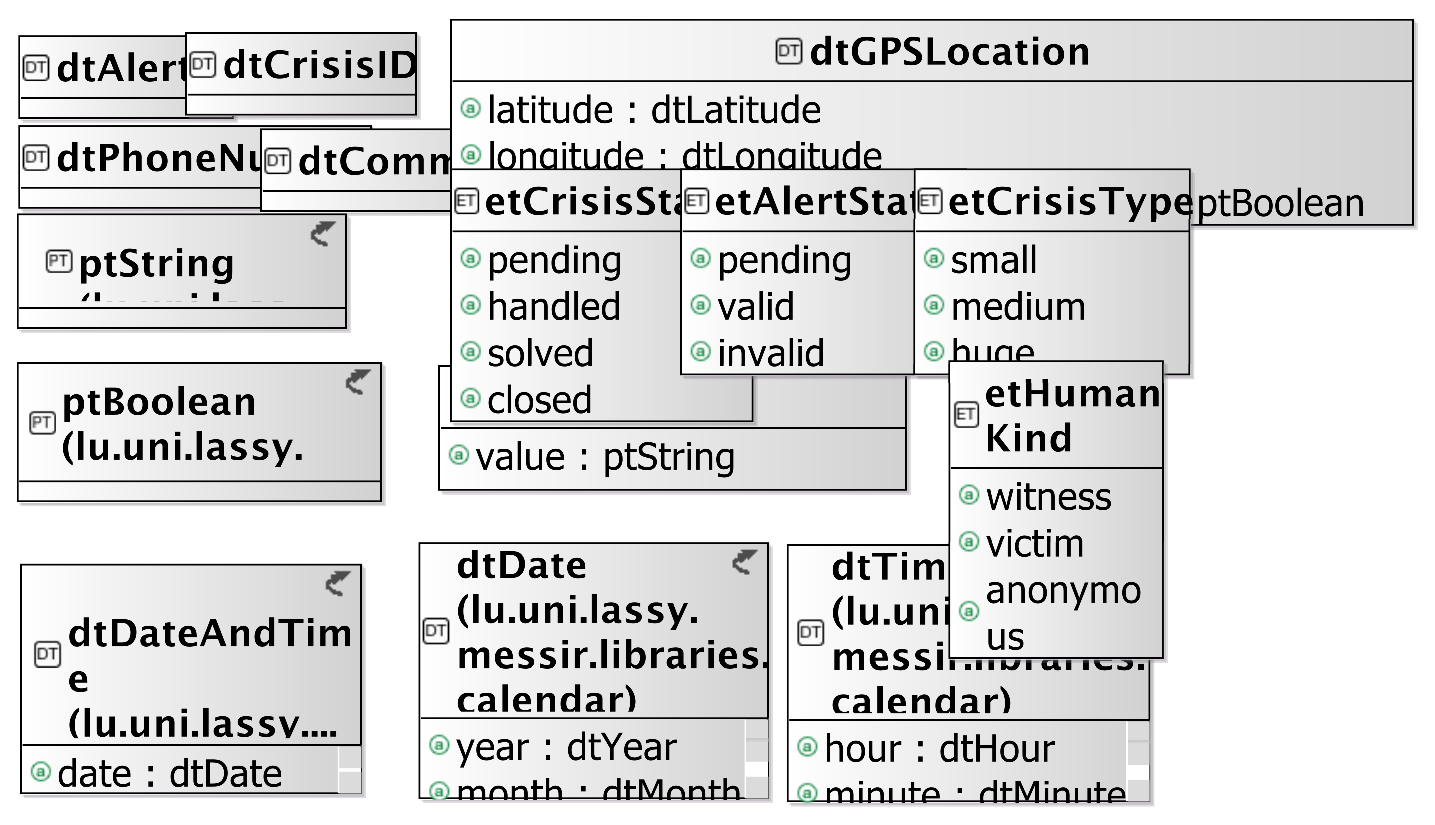
\includegraphics[
angle=0
,width=1.0\textwidth
]{./images-report-gen/operation-model/operation-scope-outactComCompany-oeAlertv2.eps}
\end{center}
\caption[lu.uni.lassy.excalibur.examples.icrash Operation Scope: operation-scope-outactComCompany-oeAlertv2]{oeAlert operation scope
}
\label{fig:lu.uni.lassy.excalibur.examples.icrash-OM-scopeView-operation-scope-outactComCompany-oeAlertv2}
\end{figure}
\vspace{0.5cm}

Figure \ref{fig:lu.uni.lassy.excalibur.examples.icrash-OM-scopeView-operation-scope-outactComCompany-oeAlertv3}
shows concept model elements in the scope of the oeAlert operation

\begin{figure}[htbp]
\begin{center}

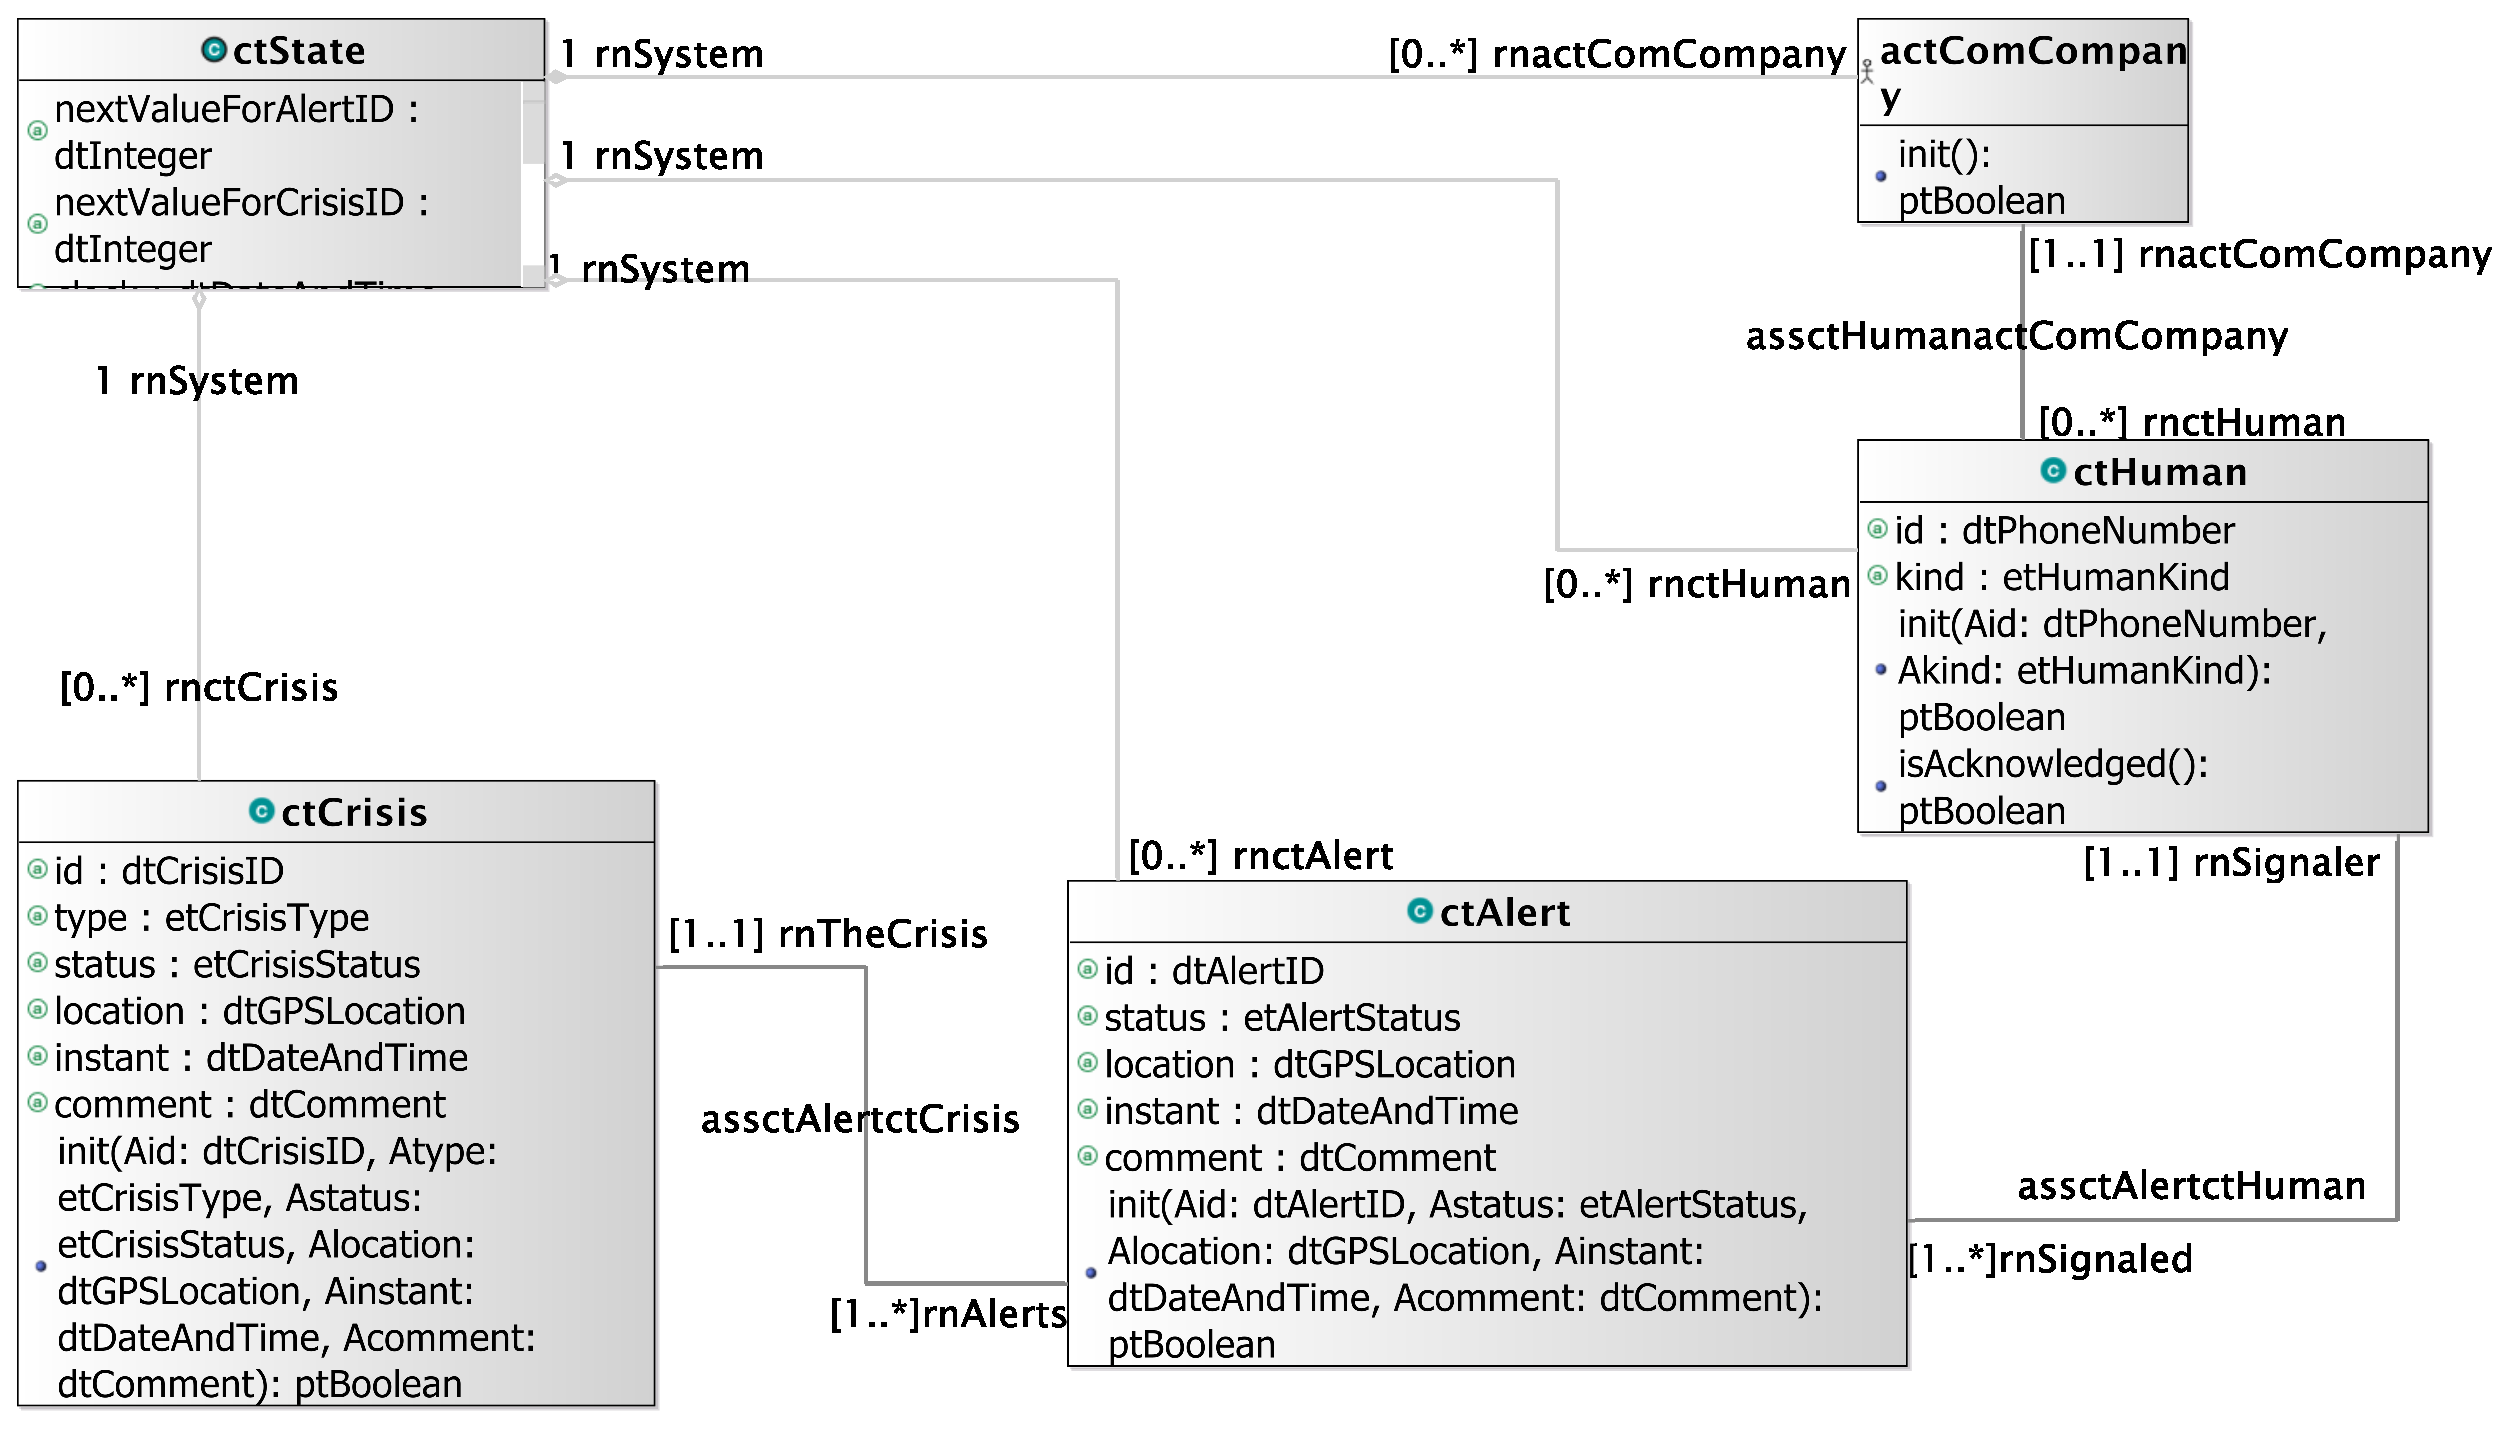
\includegraphics[
angle=0
,width=1.0\textwidth
]{./images-report-gen/operation-model/operation-scope-outactComCompany-oeAlertv3.eps}
\end{center}
\caption[lu.uni.lassy.excalibur.examples.icrash Operation Scope: operation-scope-outactComCompany-oeAlertv3]{oeAlert operation scope
}
\label{fig:lu.uni.lassy.excalibur.examples.icrash-OM-scopeView-operation-scope-outactComCompany-oeAlertv3}
\end{figure}
\vspace{0.5cm}


\section{Environment - Out Interface Operation Scheme for actCoordinator}
\label{OM-EM-OutInterface-OS-actCoordinator}
\subsection{Operation Model for oeCloseCrisis}

\label{OM-oeCloseCrisis}


The \msrcode{oeCloseCrisis} operation has the following properties:

	\begin{operationmodel}
	\addheading{Operation}
	\adddoublerow{oeCloseCrisis}{sent to indicate that a crisis should be considered as closed.}

	\addrowheading{Parameters}
	\addnumbereddoublerow{}{AdtCrisisID: dtCrisisID}{the identification information used to determine the crisis to close} 

	\addrowheading{Return type}
	\addsinglerow{ptBoolean}

	\addrowheading{Pre-Condition (protocol)}
	\addnumberedsinglerow{PreP}{the system is started}
	\addnumberedsinglerow{PreP}{the actor logged previously and did not log out ! (i.e. the associated ctCoordinator instance is considered logged)}
		
	\addrowheading{Pre-Condition (functional)}
	\addnumberedsinglerow{PreF}{it is supposed that there exist one ctCrisis instance with the same \msrcode{id} attribute value as the one provided by the coordinator actor who wants to close.}

	\addrowheading{Post-Condition (functional)}
	\addnumberedsinglerow{PostF}{the ctCrisis class instance having the provided id is considered closed in the post state.}
	\addnumberedsinglerow{PostF}{There is no handler declared in the system as associated to the crisis.}
	\addnumberedsinglerow{PostF}{all the alert instances associated to this crisis do not belong any more to the system's post state.}
	\addnumberedsinglerow{PostF}{the coordinator actor is informed about the satisfaction of its request.}

	\addrowheading{Post-Condition (protocol)}
	\addnumberedsinglerow{PostP}{none}
	\end{operationmodel}



	
	
	
	






\subsection{Operation Model for oeGetAlertsSet}

\label{OM-oeGetAlertsSet}


The \msrcode{oeGetAlertsSet} operation has the following properties:

	\begin{operationmodel}
	\addheading{Operation}
	\adddoublerow{oeGetAlertsSet}{sent to request all the ctAlert instances having a specific status.}

	\addrowheading{Parameters}
	\addnumbereddoublerow{}{AetAlertStatus: etAlertStatus}{the criteria used to select the alerts to send back to the actor} 

	\addrowheading{Return type}
	\addsinglerow{ptBoolean}

	\addrowheading{Pre-Condition (protocol)}
	\addnumberedsinglerow{PreP}{the system is started}
	\addnumberedsinglerow{PreP}{the actor logged previously and did not log out ! (i.e. the associated ctCoordinator instance is considered logged)}
		
	\addrowheading{Pre-Condition (functional)}
	\addnumberedsinglerow{PreF}{none}

	\addrowheading{Post-Condition (functional)}
	\addnumberedsinglerow{PostF}{ the post state is the one obtained by satisfying the \msrcode{isSentToCoordinator} predicate for each alert having the provided status and for the actor sending the message. (cf. specification of \msrcode{isSentToCoordinator} predicate given for the \msrcode{ctAlert} type.}

	\addrowheading{Post-Condition (protocol)}
	\addnumberedsinglerow{PostP}{ none}
	\end{operationmodel}



	
	
	
	






\subsection{Operation Model for oeGetCrisisSet}

\label{OM-oeGetCrisisSet}


The \msrcode{oeGetCrisisSet} operation has the following properties:

	\begin{operationmodel}
	\addheading{Operation}
	\adddoublerow{oeGetCrisisSet}{sent to request all the ctCrisis instances having a specific status.}

	\addrowheading{Parameters}
	\addnumbereddoublerow{}{AetCrisisStatus: etCrisisStatus}{the status information used to determine the crisis to send back to the actor} 

	\addrowheading{Return type}
	\addsinglerow{ptBoolean}

	\addrowheading{Pre-Condition (protocol)}
	\addnumberedsinglerow{PreP}{the system is started}
	\addnumberedsinglerow{PreP}{the actor logged previously and did not log out ! (i.e. the associated ctCoordinator instance is considered logged)}
		
	\addrowheading{Pre-Condition (functional)}
	\addnumberedsinglerow{PreF}{none}

	\addrowheading{Post-Condition (functional)}
	\addnumberedsinglerow{PostF}{ the post state is the one obtained by satisfying the \msrcode{isSentToCoordinator} predicate for each crisis having the provided status and for the actor sending the message \msrcode{ieSendACrisis}. (cf. specification of \msrcode{isSentToCoordinator} predicate given for the \msrcode{ctCrisis} type.}

	\addrowheading{Post-Condition (protocol)}
	\addnumberedsinglerow{PostP}{ none}
	\end{operationmodel}



	
	
	
	






\subsection{Operation Model for oeInvalidateAlert}

\label{OM-oeInvalidateAlert}


The \msrcode{oeInvalidateAlert} operation has the following properties:

	\begin{operationmodel}
	\addheading{Operation}
	\adddoublerow{oeInvalidateAlert}{ sent to indicate that an alert should be considered as closed.}

	\addrowheading{Parameters}
	\addnumbereddoublerow{}{AdtAlertID: dtAlertID}{the identification information used to determine the alert to close} 

	\addrowheading{Return type}
	\addsinglerow{ptBoolean}

	\addrowheading{Pre-Condition (protocol)}
	\addnumberedsinglerow{PreP}{the system is started}
	\addnumberedsinglerow{PreP}{the actor logged previously and did not log out ! (i.e. the associated ctCoordinator instance is considered logged)}
		
	\addrowheading{Pre-Condition (functional)}
	\addnumberedsinglerow{PreF}{ it is supposed that there exist one ctAlert instance with the same \msrcode{id} attribute value as the one provided by the coordinator actor who wants to close.}

	\addrowheading{Post-Condition (functional)}
	\addnumberedsinglerow{PostF}{the ctAlert class instance having the provided id is considered closed in the post state.}
	\addnumberedsinglerow{PostF}{the coordinator actor is informed about the satisfaction of its request.}

	\addrowheading{Post-Condition (protocol)}
	\addnumberedsinglerow{PostP}{ none}
	\end{operationmodel}



	
	
	
	






\subsection{Operation Model for oeReportOnCrisis}

\label{OM-oeReportOnCrisis}


The \msrcode{oeReportOnCrisis} operation has the following properties:

	\begin{operationmodel}
	\addheading{Operation}
	\adddoublerow{oeReportOnCrisis}{sent to update the textual information available for a specific handled crisis.}

	\addrowheading{Parameters}
	\addnumbereddoublerow{}{AdtCrisisID: dtCrisisID}{the identification information used to determine the crisis to report on} 
	\addnumbereddoublerow{}{AdtComment: dtComment}{the textual information commenting the crisis} 

	\addrowheading{Return type}
	\addsinglerow{ptBoolean}

	\addrowheading{Pre-Condition (protocol)}
	\addnumberedsinglerow{PreP}{the system is started}
	\addnumberedsinglerow{PreP}{the actor logged previously and did not log out ! (i.e. the associated ctCoordinator instance is considered logged)}
		
	\addrowheading{Pre-Condition (functional)}
	\addnumberedsinglerow{PreF}{it is supposed that there exist one crisis in the pre state having the given id.}

	\addrowheading{Post-Condition (functional)}
	\addnumberedsinglerow{PostF}{the comment attribute of the crisis instance having the given id is replaced by the given one and the requesting actor is notified of this update.}

	\addrowheading{Post-Condition (protocol)}
	\addnumberedsinglerow{PostP}{ none}
	\end{operationmodel}



	
	
	
	






\subsection{Operation Model for oeSetCrisisHandler}

\label{OM-oeSetCrisisHandler}


The \msrcode{oeSetCrisisHandler} operation has the following properties:

	\begin{operationmodel}
	\addheading{Operation}
	\adddoublerow{oeSetCrisisHandler}{sent to declare himself as been the handler of a crisis having the specified id.}

	\addrowheading{Parameters}
	\addnumbereddoublerow{}{AdtCrisisID: dtCrisisID}{the identification information used to determine the crisis} 

	\addrowheading{Return type}
	\addsinglerow{ptBoolean}

	\addrowheading{Pre-Condition (protocol)}
	\addnumberedsinglerow{PreP}{the system is started}
	\addnumberedsinglerow{PreP}{the actor logged previously and did not log out ! (i.e. the associated ctCoordinator instance is considered logged)}
		
	\addrowheading{Pre-Condition (functional)}
	\addnumberedsinglerow{PreF}{ there exist one crisis having the given id in the pre-state.}

	\addrowheading{Post-Condition (functional)}
	\addnumberedsinglerow{PostF}{the ctCrisis instance having the provided id is in handled status at poststate and is associated to the actor that sends the message (which himself is notified with a textual message as confirmation).}
	\addnumberedsinglerow{PostF}{All the alerts related to this crisis are sent to the actor such that he can decide how to handle them.}
	\addnumberedsinglerow{PostF}{if the crisis was already handled at pre-sate then the associated handler actor is notified about the change of handler for one of his crisis (n.b. it might be the same even if not relevant).}
	\addnumberedsinglerow{PostF}{a message is sent to the communication company for any human related to an alert associated to the crisis. A human will receive as many messages as alerts he sent despite the fact that they might relate to the same crisis (i.e. one alert, one acknoledgement).}

	\addrowheading{Post-Condition (protocol)}
	\addnumberedsinglerow{PostP}{ none}
	\end{operationmodel}



	
	
	
	






\subsection{Operation Model for oeSetCrisisStatus}

\label{OM-oeSetCrisisStatus}


The \msrcode{oeSetCrisisStatus} operation has the following properties:

	\begin{operationmodel}
	\addheading{Operation}
	\adddoublerow{oeSetCrisisStatus}{sent to define the handling status of a specific crisis.}

	\addrowheading{Parameters}
	\addnumbereddoublerow{}{AdtCrisisID: dtCrisisID}{the identification information used to determine the crisis} 
	\addnumbereddoublerow{}{AetCrisisStatus: etCrisisStatus}{the new status value} 

	\addrowheading{Return type}
	\addsinglerow{ptBoolean}

	\addrowheading{Pre-Condition (protocol)}
	\addnumberedsinglerow{PreP}{the system is started}
	\addnumberedsinglerow{PreP}{the actor logged previously and did not log out ! (i.e. the associated ctCoordinator instance is considered logged)}
		
	\addrowheading{Pre-Condition (functional)}
	\addnumberedsinglerow{PreF}{it is supposed that there exist one crisis in the pre state having the given id.}

	\addrowheading{Post-Condition (functional)}
	\addnumberedsinglerow{PostF}{the crisis status attribute of the crisis instance having the given id is replaced by the given one and the requesting actor is notified of this update.}

	\addrowheading{Post-Condition (protocol)}
	\addnumberedsinglerow{PostP}{none}
	\end{operationmodel}



	
	
	
	






\subsection{Operation Model for oeSetCrisisType}

\label{OM-oeSetCrisisType}


The \msrcode{oeSetCrisisType} operation has the following properties:

	\begin{operationmodel}
	\addheading{Operation}
	\adddoublerow{oeSetCrisisType}{sent to define the gravity type of a specific crisis.}

	\addrowheading{Parameters}
	\addnumbereddoublerow{}{AdtCrisisID: dtCrisisID}{the identification information used to determine the crisis} 
	\addnumbereddoublerow{}{AetCrisisType: etCrisisType}{the new type value} 

	\addrowheading{Return type}
	\addsinglerow{ptBoolean}

	\addrowheading{Pre-Condition (protocol)}
	\addnumberedsinglerow{PreP}{the system is started}
	\addnumberedsinglerow{PreP}{the actor logged previously and did not log out ! (i.e. the associated ctCoordinator instance is considered logged)}
		
	\addrowheading{Pre-Condition (functional)}
	\addnumberedsinglerow{PreF}{it is supposed that there exist one crisis in the pre state having the given id.}

	\addrowheading{Post-Condition (functional)}
	\addnumberedsinglerow{PostF}{the crisis type attribute of the crisis instance having the given id is replaced by the given one and the requesting actor is notified of this update.}

	\addrowheading{Post-Condition (protocol)}
	\addnumberedsinglerow{PostP}{none}
	\end{operationmodel}



	
	
	
	






\subsection{Operation Model for oeValidateAlert}

\label{OM-oeValidateAlert}


The \msrcode{oeValidateAlert} operation has the following properties:

	\begin{operationmodel}
	\addheading{Operation}
	\adddoublerow{oeValidateAlert}{sent to indicate that a specific alert is not a fake.}

	\addrowheading{Parameters}
	\addnumbereddoublerow{}{AdtAlertID: dtAlertID}{the identification information used to determine the alert instance} 

	\addrowheading{Return type}
	\addsinglerow{ptBoolean}

	\addrowheading{Pre-Condition (protocol)}
	\addnumberedsinglerow{PreP}{the system is started}
	\addnumberedsinglerow{PreP}{the actor logged previously and did not log out ! (i.e. the associated ctCoordinator instance is considered logged)}
		
	\addrowheading{Pre-Condition (functional)}
	\addnumberedsinglerow{PreF}{ it is supposed that there exist one ctAlert instance with the same \msrcode{id} attribute value as the one provided by the coordinator actor who wants to validate.}

	\addrowheading{Post-Condition (functional)}
	\addnumberedsinglerow{PostF}{the ctAlert class instance having the provided id is considered as valid in the post state and the coordinator actor is informed about the satisfaction of its request.}

	\addrowheading{Post-Condition (protocol)}
	\addnumberedsinglerow{PostP}{ none}
	\end{operationmodel}



	
	
	
	






\section{Environment - Out Interface Operation Scheme for actMsrCreator}
\label{OM-EM-OutInterface-OS-actMsrCreator}
\subsection{Operation Model for oeCreateSystemAndEnvironment}

\label{OM-oeCreateSystemAndEnvironment}


The \msrcode{oeCreateSystemAndEnvironment} operation has the following properties:

	\begin{operationmodel}
	\addheading{Operation}
	\adddoublerow{oeCreateSystemAndEnvironment}{sent to request the initialization of the system's class instances and the environment actors instances.}

	\addrowheading{Parameters}
	\addnumbereddoublerow{}{AqtyComCompanies: ptInteger}{the quantity of communication companies to create in the environment} 

	\addrowheading{Return type}
	\addsinglerow{ptBoolean}

	\addrowheading{Pre-Condition (protocol)}
	\addnumberedsinglerow{PreP}{ none}
		
	\addrowheading{Pre-Condition (functional)}
	\addnumberedsinglerow{PreF}{ none }

	\addrowheading{Post-Condition (functional)}
	\addnumberedsinglerow{PostF}{ the ctState instance is initialized with the integer 1 for the crisis and alert counters used for their identifications, a value for the clock corresponding to a default inital time (i.e. January 1st, 1970) the crisis reminder period is set to 300 seconds, the maximum crisis reminder period is fixed to 1200 seconds (i.e. 20 minutes), an initial value for the automatic reminder period equal to the current date and time and the system is considered in a started state.
	
	{\bf Those predicates must be satisfied first since all the other depend on the existence of a ctState instance !}}
	\addnumberedsinglerow{PostF}{the \msrcode{actMsrCreator} actor instance is initiated (remember that since the \msrcode{oeCreateSystemAndEnvironment} is a special event it role is to make consistent the post state thus creating the actor and its interfaces is required even though the sending of this message logically would need the actor and its interfaces to already exist ...).}
	\addnumberedsinglerow{PostF}{the environment for communication company actors, in the post state, is made of \msrcode{AqtyComCompanies} instances allowing for receiving and sending messages to humans.}
	\addnumberedsinglerow{PostF}{the environment for administrator actors, in the post state, is made of one instance.}
	\addnumberedsinglerow{PostF}{the environment for activator actors, in the post state, is made of one instance allowing for automatic message sending based on current system's and environment state'.}
	\addnumberedsinglerow{PostF}{the set of ctAdministrator instances at post is made of one instance initialized with 'icrashadmin' (resp. '7WXC1359') for login (resp. password) values.}
	\addnumberedsinglerow{PostF}{the association between ctAdministrator and actAdministrator is made of one couple made of the conjointly specified instances.}

	\addrowheading{Post-Condition (protocol)}
	\addnumberedsinglerow{PostP}{ none is given since the only protocol variable to be modified in the post state is the one initialized with the ctState instance (i.e. vpStarted).}
	\end{operationmodel}



	% ------------------------------------------
	% MCL Listing
	% ------------------------------------------
	\vspace{1cm}
	The listing~\ref{OM-actMsrCreator-oeCreateSystemAndEnvironment-MCL-LST} provides the \msrmessir (MCL-oriented) specification of the operation.
	
	\scriptsize
	\vspace{0.5cm}
	\begin{lstlisting}[style=MessirStyle,firstnumber=auto,captionpos=b,caption={\msrmessir (MCL-oriented) specification of the operation \emph{oeCreateSystemAndEnvironment}.},label=OM-actMsrCreator-oeCreateSystemAndEnvironment-MCL-LST]

	/* Pre Protocol:*/ 
	preP{true}
	
	/* Pre Functional:*/
	preF{true}
	
	/* Post Functional:*/ 
	postF{let TheSystem: ctState in
	  let AactMsrCreator: actMsrCreator in
	  let AactAdministrator: actAdministrator in
	  let AnextValueForAlertID: dtInteger in
	  let AnextValueForCrisisID: dtInteger in
	  let Aclock: dtDateAndTime in
	  let AcrisisReminderPeriod: dtSecond in
	  let AmaxCrisisReminderPeriod: dtSecond in
	  let AvpStarted: ptBoolean in
	
	  /* PostF01 -- MUST ALWAYS BE MADE FIRST -- */ 
	  AnextValueForAlertID.value.eq(1)
	  and AnextValueForCrisisID.value.eq(1)
	  and Aclock.date.year.value = 1970 
	  and Aclock.date.month.value = 01
	  and Aclock.date.day.value = 01
	  and Aclock.time.hour.value = 00
	  and Aclock.time.minute.value = 00
	  and Aclock.time.second.value = 00
	
	  and AcrisisReminderPeriod.value.eq(300)
	  and AmaxCrisisReminderPeriod.value.eq(1200)
	  and AvpStarted = true
	  and TheSystem.init(AnextValueForAlertID,
	                     AnextValueForCrisisID,
	                     Aclock,
	                     AcrisisReminderPeriod,
	                     AmaxCrisisReminderPeriod,
	                     Aclock,
	                     AvpStarted
	                    )
	  /* PostF02*/ 
	  and AactMsrCreator.init()
	  /* PostF03 */ 
	  and let AactComCompanyCol: Bag(actComCompany) in
	  AactComCompanyCol->size() = AqtyComCompanies
	  AactComCompanyCol-> forAll(init())
	 /* PostF04*/ 
	  and AactAdministrator.init()
	  /* PostF05*/ 
	  and let AactActivator:actActivator in
	  AactActivator.init()
	/* PostF06 */ 
	  and let ActAdministrator:ctAdministrator in
	      let AdtLogin:dtLogin in
	      let AdtPassword:dtPassword in
	      AdtLogin.value.eq('icrashadmin')
	      and AdtPassword.value.eq('7WXC1359')
	      and ActAdministrator.init(AdtLogin,AdtPassword)
	 /* PostF07*/ 
	  and ActAdministrator@post.rnactAuthenticated = AactAdministrator}
	
	/* Post Protocol:*/ 
	postP{ true}
	
	\end{lstlisting}
	\normalsize 
	
	
	
	





Figure \ref{fig:lu.uni.lassy.excalibur.examples.icrash-OM-scopeView-operation-scope-outactMsrCreator-oeCreateSystemAndEnvironment}
shows all the concept model elements in the scope of the oeCreateSystemAndEnvironment operation

\begin{figure}[htbp]
\begin{center}

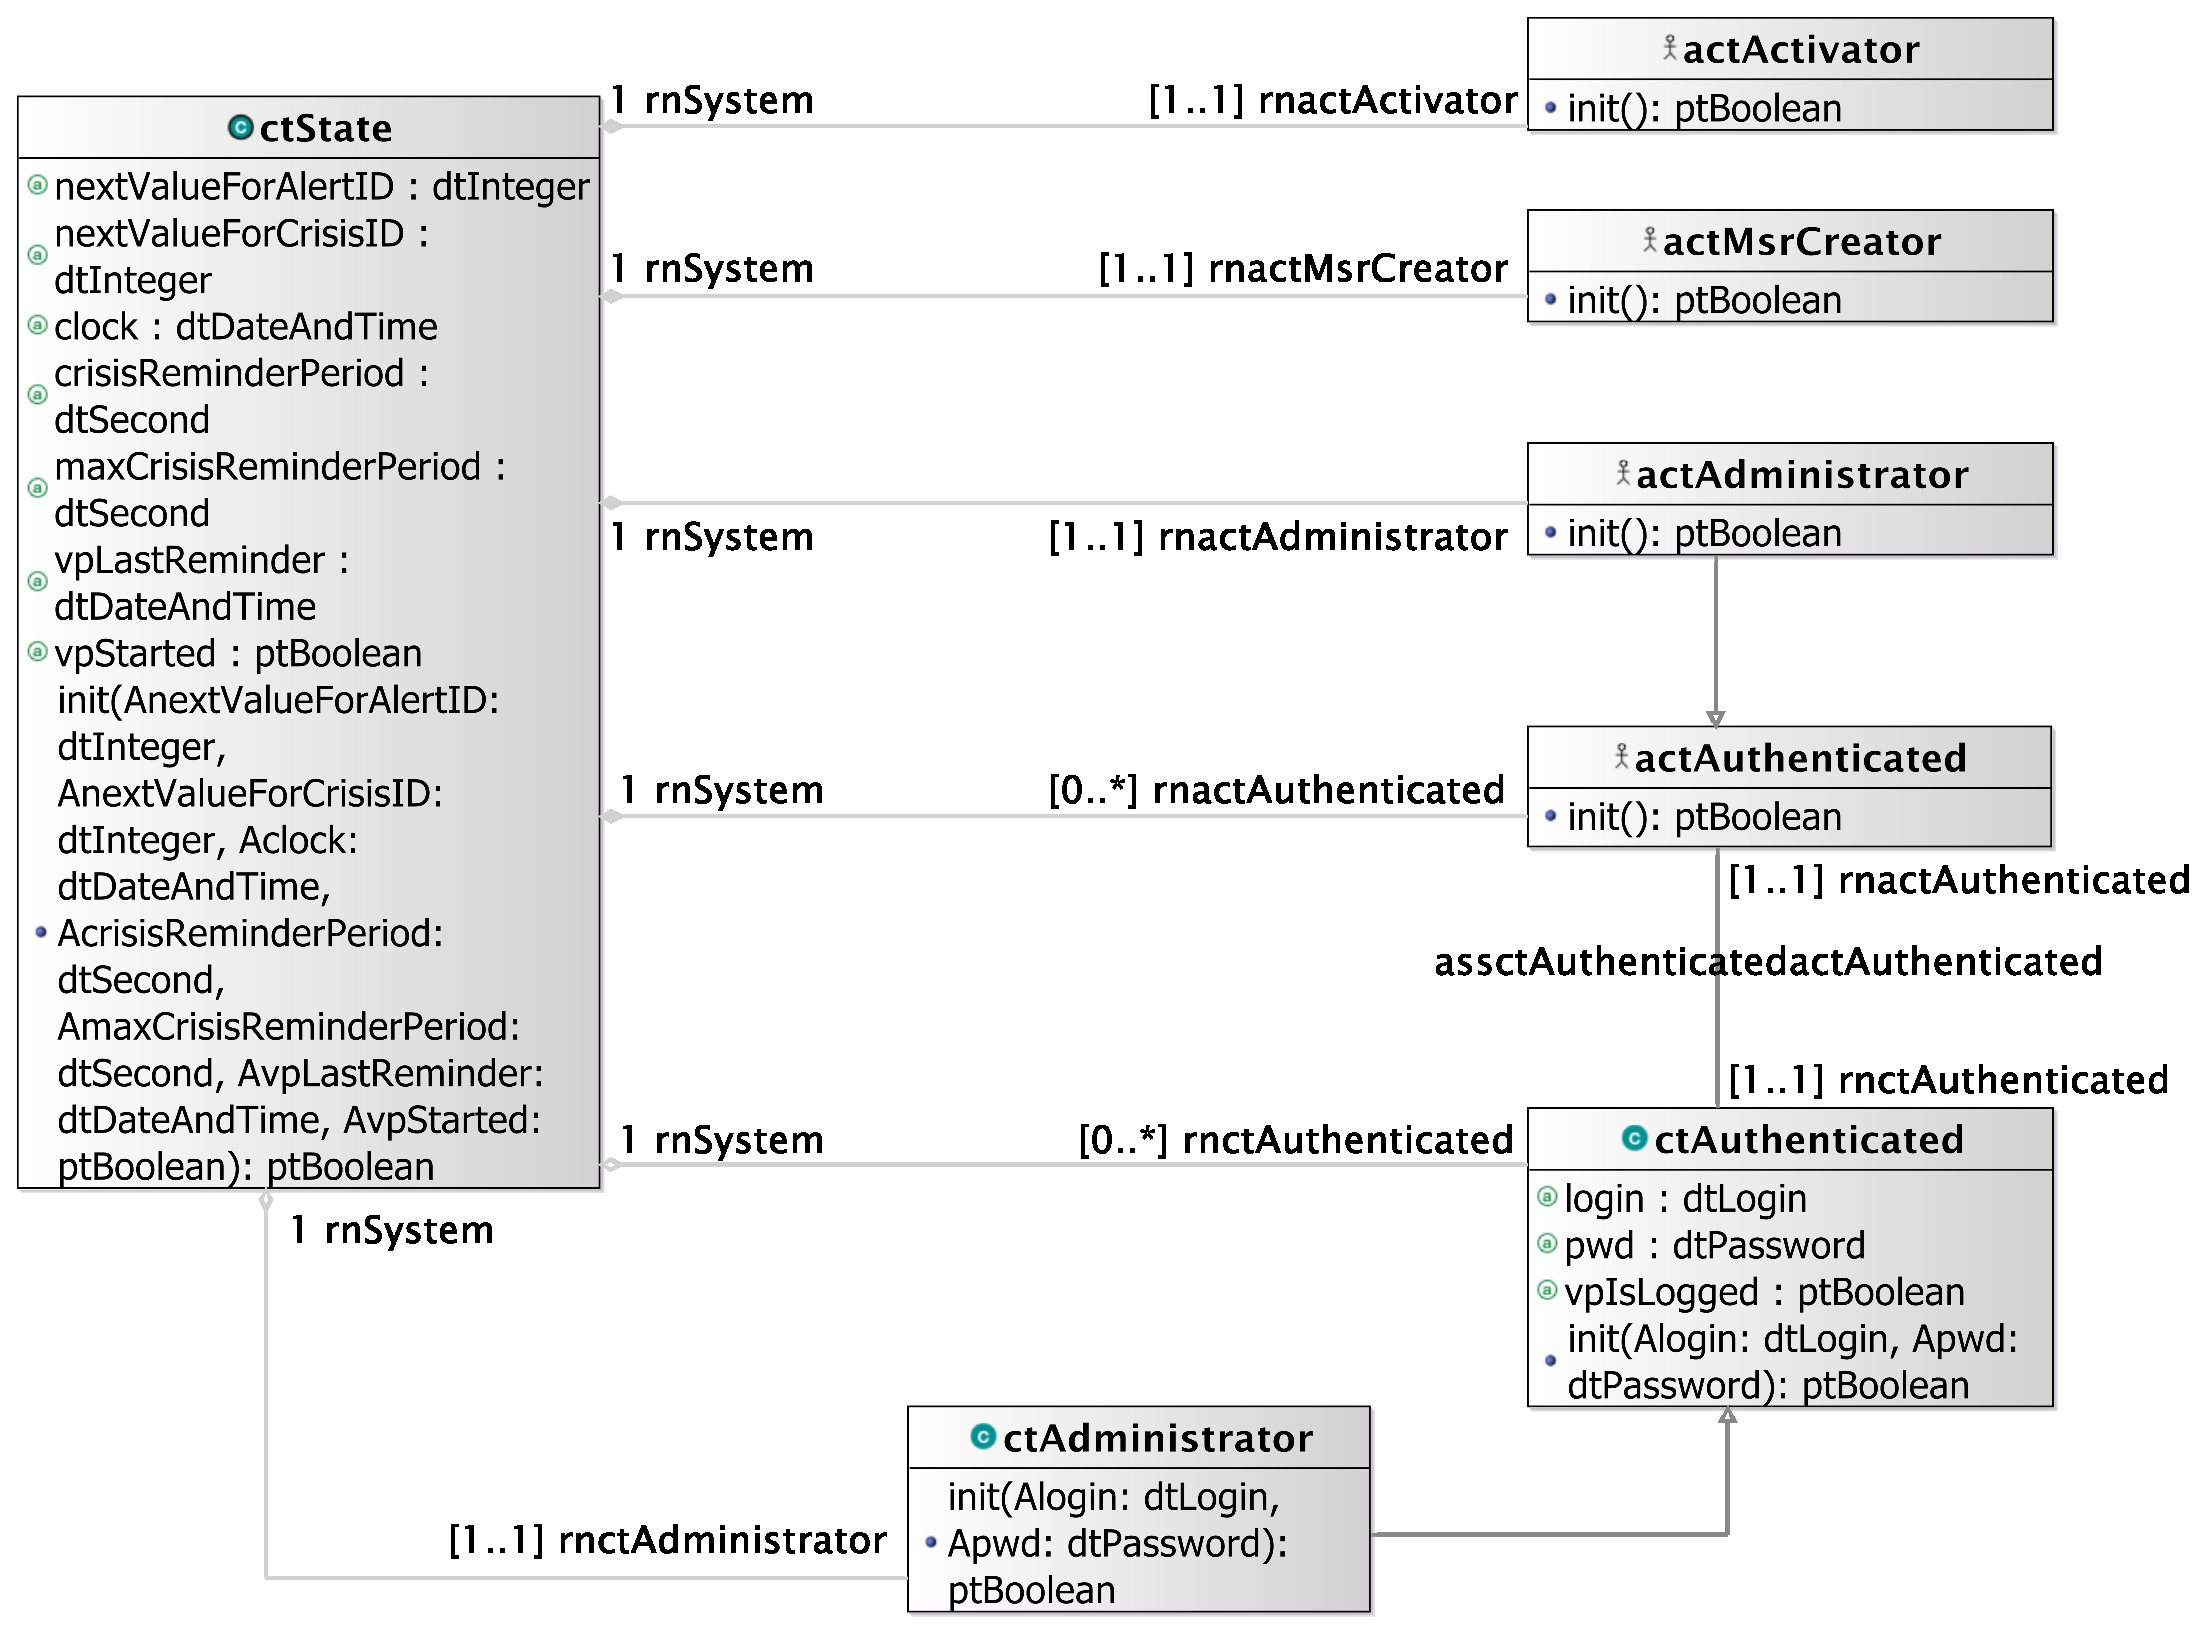
\includegraphics[
angle=0
,width=1.0\textwidth
]{./images-report-gen/operation-model/operation-scope-outactMsrCreator-oeCreateSystemAndEnvironment.eps}
\end{center}
\caption[lu.uni.lassy.excalibur.examples.icrash Operation Scope: operation-scope-outactMsrCreator-oeCreateSystemAndEnvironment]{oeCreateSystemAndEnvironment operation scope
}
\label{fig:lu.uni.lassy.excalibur.examples.icrash-OM-scopeView-operation-scope-outactMsrCreator-oeCreateSystemAndEnvironment}
\end{figure}
\vspace{0.5cm}



%% ***************************************************************
%% operations for: Environment-Actor Operation Schemes

		
\section{Environment - Actor Operation Scheme for actMsrCreator}
\label{OM-EM-actMsrCreator}
\subsection{Operation Model for init}

\label{OM-init}


The \msrcode{init} operation has the following properties:

	\begin{operationmodel}
	\addheading{Operation}
	\adddoublerow{init}{used to create an instance of the actor together with its interface instances and update the assocations with the \msrcode{ctState} instance.}


	\addrowheading{Return type}
	\addsinglerow{ptBoolean}

		


	\end{operationmodel}



	
	
	
	





 

%% ***************************************************************
%% operations for primary type classes


\section{Primary Types - Operation Schemes for Class ctAdministrator} 
\label{OM-CM-PTClass-ctAdministrator}
\subsection{Operation Model for init}

\label{OM-init}


The \msrcode{init} operation has the following properties:

	\begin{operationmodel}
	\addheading{Operation}
	\adddoublerow{init}{ used to initialize the current object as a new instance of the ctAdministrator type.}

	\addrowheading{Parameters}
	\addnumbereddoublerow{}{Alogin: dtLogin}{used to initialize the login field} 
	\addnumbereddoublerow{}{Apwd: dtPassword}{used to initialize the password field} 

	\addrowheading{Return type}
	\addsinglerow{ptBoolean}

		

	\addrowheading{Post-Condition (functional)}
	\addnumberedsinglerow{PostF}{ 
	true iff the system poststate includes the current object as a new ctAdministrator instance having its login and password attributes equal to the one provided as parameters and its vpIsLogged attribute equal to false. }

	\end{operationmodel}



	% ------------------------------------------
	% MCL Listing
	% ------------------------------------------
	\vspace{1cm}
	The listing~\ref{OM-ctAdministrator-init-MCL-LST} provides the \msrmessir (MCL-oriented) specification of the operation.
	
	\scriptsize
	\vspace{0.5cm}
	\begin{lstlisting}[style=MessirStyle,firstnumber=auto,captionpos=b,caption={\msrmessir (MCL-oriented) specification of the operation \emph{init}.},label=OM-ctAdministrator-init-MCL-LST]

	
	
	/* Post Functional:*/ 
	postF{if
	(
	let Self:ctAdministrator in
	/* Post F01 */
	Self.login(Alogin)
	and Self.pwd = Apwd
	and Self.vpIsLogged = false
	
	/* Post F02 */
	and (Self.oclIsNew and self = Self)
	)
	then (result = true)
	else (result = false)
	endif}
	
	
	\end{lstlisting}
	\normalsize 
	
	
	
	






\section{Primary Types - Operation Schemes for Class ctAlert} 
\label{OM-CM-PTClass-ctAlert}
\subsection{Operation Model for init}

\label{OM-init}


The \msrcode{init} operation has the following properties:

	\begin{operationmodel}
	\addheading{Operation}
	\adddoublerow{init}{ used to initialize the current object as a new instance of the ctAlert type.}

	\addrowheading{Parameters}
	\addnumbereddoublerow{}{Aid: dtAlertID}{used to initialize the id field} 
	\addnumbereddoublerow{}{Astatus: etAlertStatus}{used to initialize the status field} 
	\addnumbereddoublerow{}{Alocation: dtGPSLocation}{used to initialize the location field} 
	\addnumbereddoublerow{}{Ainstant: dtDateAndTime}{used to initialize the instant field} 
	\addnumbereddoublerow{}{Acomment: dtComment}{used to initialize the comment field} 

	\addrowheading{Return type}
	\addsinglerow{ptBoolean}

		

	\addrowheading{Post-Condition (functional)}
	\addnumberedsinglerow{PostF}{true iff the system poststate includes the current object as a new ctAlert instance having its attributes equal to the ones provided as parameters. 
	}

	\end{operationmodel}



	% ------------------------------------------
	% MCL Listing
	% ------------------------------------------
	\vspace{1cm}
	The listing~\ref{OM-ctAlert-init-MCL-LST} provides the \msrmessir (MCL-oriented) specification of the operation.
	
	\scriptsize
	\vspace{0.5cm}
	\begin{lstlisting}[style=MessirStyle,firstnumber=auto,captionpos=b,caption={\msrmessir (MCL-oriented) specification of the operation \emph{init}.},label=OM-ctAlert-init-MCL-LST]

	
	
	/* Post Functional:*/ 
	postF{if
	(
	/* Post F01 */
	let Self:ctAlert in
	Self.id = Aid
	and Self.status = Astatus
	and Self.location = Alocation
	and Self.instant = Ainstant
	and Self.comment = Acomment
	/* Post F02 */
	and (Self.oclIsNew and self = Self)
	)
	then (result = true)
	else (result = false)
	endif}
	
	
	\end{lstlisting}
	\normalsize 
	
	
	
	






\subsection{Operation Model for isSentToCoordinator}

\label{OM-isSentToCoordinator}


The \msrcode{isSentToCoordinator} operation has the following properties:

	\begin{operationmodel}
	\addheading{Operation}
	\adddoublerow{isSentToCoordinator}{ used to provide a given coordinator with current alert information.}

	\addrowheading{Parameters}
	\addnumbereddoublerow{}{AactCoordinator: actCoordinator}{the message destination} 

	\addrowheading{Return type}
	\addsinglerow{ptBoolean}

		

	\addrowheading{Post-Condition (functional)}
	\addnumberedsinglerow{PostF}{ true iff the message ieSendAnAlert is sent to the input interface of the given coordinator actor with the current alert as parameter value.}

	\end{operationmodel}



	% ------------------------------------------
	% MCL Listing
	% ------------------------------------------
	\vspace{1cm}
	The listing~\ref{OM-ctAlert-isSentToCoordinator-MCL-LST} provides the \msrmessir (MCL-oriented) specification of the operation.
	
	\scriptsize
	\vspace{0.5cm}
	\begin{lstlisting}[style=MessirStyle,firstnumber=auto,captionpos=b,caption={\msrmessir (MCL-oriented) specification of the operation \emph{isSentToCoordinator}.},label=OM-ctAlert-isSentToCoordinator-MCL-LST]

	
	
	/* Post Functional:*/ 
	postF{if
	(
	/* Post F01 */
	AactCoordinator.rnInterfaceIN.ieSendAnAlert(self)
	)
	then (result = true)
	else (result = false)
	endif}
	
	
	\end{lstlisting}
	\normalsize 
	
	
	
	






\section{Primary Types - Operation Schemes for Class ctAuthenticated} 
\label{OM-CM-PTClass-ctAuthenticated}
\subsection{Operation Model for init}

\label{OM-init}


The \msrcode{init} operation has the following properties:

	\begin{operationmodel}
	\addheading{Operation}
	\adddoublerow{init}{used to initialize the current object as a new instance of the ctAuthenticated type.}

	\addrowheading{Parameters}
	\addnumbereddoublerow{}{Alogin: dtLogin}{used to initialize the login field} 
	\addnumbereddoublerow{}{Apwd: dtPassword}{used to initialize the password field} 

	\addrowheading{Return type}
	\addsinglerow{ptBoolean}

		

	\addrowheading{Post-Condition (functional)}
	\addnumberedsinglerow{PostF}{true iff the system poststate includes the current object as a new ctAuthenticated instance having its attributes equal to the ones provided as parameters.}

	\end{operationmodel}



	
	
	
	






\section{Primary Types - Operation Schemes for Class ctCoordinator} 
\label{OM-CM-PTClass-ctCoordinator}
\subsection{Operation Model for init}

\label{OM-init}


The \msrcode{init} operation has the following properties:

	\begin{operationmodel}
	\addheading{Operation}
	\adddoublerow{init}{used to initialize the current object as a new instance of the ctCoordinator type.}

	\addrowheading{Parameters}
	\addnumbereddoublerow{}{Aid: dtCoordinatorID}{used to initialize the id field} 
	\addnumbereddoublerow{}{Alogin: dtLogin}{used to initialize the login field} 
	\addnumbereddoublerow{}{Apwd: dtPassword}{used to initialize the password field} 

	\addrowheading{Return type}
	\addsinglerow{ptBoolean}

		

	\addrowheading{Post-Condition (functional)}
	\addnumberedsinglerow{PostF}{true iff the system poststate includes the current object as a new ctCoordinator instance having its attributes equal to the ones provided as parameters.
	 }

	\end{operationmodel}



	% ------------------------------------------
	% MCL Listing
	% ------------------------------------------
	\vspace{1cm}
	The listing~\ref{OM-ctCoordinator-init-MCL-LST} provides the \msrmessir (MCL-oriented) specification of the operation.
	
	\scriptsize
	\vspace{0.5cm}
	\begin{lstlisting}[style=MessirStyle,firstnumber=auto,captionpos=b,caption={\msrmessir (MCL-oriented) specification of the operation \emph{init}.},label=OM-ctCoordinator-init-MCL-LST]

	
	
	/* Post Functional:*/ 
	postF{if
	(
	/* Post F01 */
	let Self:ctCoordinator in
	Self.id = Aid
	and Self.login = Alogin
	and Self.pwd = Apwd
	and Self.vpIsLogged = false
	/* Post F02 */
	and (Self.oclIsNew and self = Self)
	)
	then (result = true)
	else (result = false)
	endif}
	
	
	\end{lstlisting}
	\normalsize 
	
	
	
	






\section{Primary Types - Operation Schemes for Class ctCrisis} 
\label{OM-CM-PTClass-ctCrisis}
\subsection{Operation Model for init}

\label{OM-init}


The \msrcode{init} operation has the following properties:

	\begin{operationmodel}
	\addheading{Operation}
	\adddoublerow{init}{ used to initialize the current object as a new instance of the ctCrisis type.}

	\addrowheading{Parameters}
	\addnumbereddoublerow{}{Aid: dtCrisisID}{used to initialize the id field} 
	\addnumbereddoublerow{}{Atype: etCrisisType}{used to initialize the type field} 
	\addnumbereddoublerow{}{Astatus: etCrisisStatus}{used to initialize the status field} 
	\addnumbereddoublerow{}{Alocation: dtGPSLocation}{used to initialize the location field} 
	\addnumbereddoublerow{}{Ainstant: dtDateAndTime}{used to initialize the instant field} 
	\addnumbereddoublerow{}{Acomment: dtComment}{used to initialize the comment field} 

	\addrowheading{Return type}
	\addsinglerow{ptBoolean}

		

	\addrowheading{Post-Condition (functional)}
	\addnumberedsinglerow{PostF}{true iff the system poststate includes the current object as a new ctCrisis instance having its attributes equal to the ones provided as parameters.
	}

	\end{operationmodel}



	% ------------------------------------------
	% MCL Listing
	% ------------------------------------------
	\vspace{1cm}
	The listing~\ref{OM-ctCrisis-init-MCL-LST} provides the \msrmessir (MCL-oriented) specification of the operation.
	
	\scriptsize
	\vspace{0.5cm}
	\begin{lstlisting}[style=MessirStyle,firstnumber=auto,captionpos=b,caption={\msrmessir (MCL-oriented) specification of the operation \emph{init}.},label=OM-ctCrisis-init-MCL-LST]

	
	
	/* Post Functional:*/ 
	postF{if
	(
	/* Post F01 */
	let Self:ctCrisis in
	Self.id = Aid
	and Self.type = Atype
	and Self.status = Astatus
	and Self.location = Alocation
	and Self.instant = Ainstant
	and Self.comment = Acomment
	/* Post F02 */
	and (Self.oclIsNew and self = Self)
	)
	then (result = true)
	else (result = false)
	endif}
	
	
	\end{lstlisting}
	\normalsize 
	
	
	
	






\subsection{Operation Model for handlingDelayPassed}

\label{OM-handlingDelayPassed}


The \msrcode{handlingDelayPassed} operation has the following properties:

	\begin{operationmodel}
	\addheading{Operation}
	\adddoublerow{handlingDelayPassed}{used to determine if the crisis stood too longly in a pending status since last reminder.}


	\addrowheading{Return type}
	\addsinglerow{ptBoolean}

		

	\addrowheading{Post-Condition (functional)}
	\addnumberedsinglerow{PostF}{true iff the crisis is in pending status and if the duration between the current ctState clock information and the last reminder is greater than the crisis reminder period duration.}

	\end{operationmodel}



	% ------------------------------------------
	% MCL Listing
	% ------------------------------------------
	\vspace{1cm}
	The listing~\ref{OM-ctCrisis-handlingDelayPassed-MCL-LST} provides the \msrmessir (MCL-oriented) specification of the operation.
	
	\scriptsize
	\vspace{0.5cm}
	\begin{lstlisting}[style=MessirStyle,firstnumber=auto,captionpos=b,caption={\msrmessir (MCL-oriented) specification of the operation \emph{handlingDelayPassed}.},label=OM-ctCrisis-handlingDelayPassed-MCL-LST]

	
	
	/* Post Functional:*/ 
	postF{let TheSystem:ctState in
	let CurrentClockSecondsQty:dtInteger in
	let vpLastReminderSecondsQty:dtInteger in
	let CrisisReminderPeriod:dtSecond in
	if 
	( /* Post F01 */
	  self.rnSystem = TheSystem
	  and self.status = pending
	  and TheSystem.clock.toSecondsQty() = CurrentClockSecondsQty
	  and TheSystem.vpLastReminder.toSecondsQty() = vpLastReminderSecondsQty
	  and TheSystem.crisisReminderPeriod = CrisisReminderPeriod
	  and CurrentClockSecondsQty.sub(vpLastReminderSecondsQty).gt(CrisisReminderPeriod) = true
	)
	then (result = true)
	else (result = false)
	endif}
	
	
	\end{lstlisting}
	\normalsize 
	
	
	
	






\subsection{Operation Model for maxHandlingDelayPassed}

\label{OM-maxHandlingDelayPassed}


The \msrcode{maxHandlingDelayPassed} operation has the following properties:

	\begin{operationmodel}
	\addheading{Operation}
	\adddoublerow{maxHandlingDelayPassed}{used to determine if the crisis stood too longly in a pending status since its creation.}


	\addrowheading{Return type}
	\addsinglerow{ptBoolean}

		

	\addrowheading{Post-Condition (functional)}
	\addnumberedsinglerow{PostF}{ true iff the crisis is in pending status and if the duration between the current ctState clock information and the crisis instant is greater than the maximum reminder period duration.}

	\end{operationmodel}



	% ------------------------------------------
	% MCL Listing
	% ------------------------------------------
	\vspace{1cm}
	The listing~\ref{OM-ctCrisis-maxHandlingDelayPassed-MCL-LST} provides the \msrmessir (MCL-oriented) specification of the operation.
	
	\scriptsize
	\vspace{0.5cm}
	\begin{lstlisting}[style=MessirStyle,firstnumber=auto,captionpos=b,caption={\msrmessir (MCL-oriented) specification of the operation \emph{maxHandlingDelayPassed}.},label=OM-ctCrisis-maxHandlingDelayPassed-MCL-LST]

	
	
	/* Post Functional:*/ 
	postF{let TheSystem:ctState in
	let CurrentClockSecondsQty:dtInteger in
	let CrisisInstantSecondsQty:dtInteger in
	let MaxCrisisReminderPeriod:dtSecond in
	if 
	( /* Post F01 */
	  self.rnSystem = TheSystem
	  and self.status = pending
	  and TheSystem.clock.toSecondsQty() = CurrentClockSecondsQty
	  and Self.instant.toSecondsQty() = CrisisInstantSecondsQty
	  and TheSystem.maxCrisisReminderPeriod = MaxCrisisReminderPeriod
	  and CurrentClockSecondsQty.sub(CrisisInstantSecondsQty)
	                            .gt(MaxCrisisReminderPeriod)
	)
	then (result = true)
	else (result = false)
	endif}
	
	
	\end{lstlisting}
	\normalsize 
	
	
	
	






\subsection{Operation Model for isSentToCoordinator}

\label{OM-isSentToCoordinator}


The \msrcode{isSentToCoordinator} operation has the following properties:

	\begin{operationmodel}
	\addheading{Operation}
	\adddoublerow{isSentToCoordinator}{used to provide a given coordinator with current crisis information.}

	\addrowheading{Parameters}
	\addnumbereddoublerow{}{AactCoordinator: actCoordinator}{the message destination actor} 

	\addrowheading{Return type}
	\addsinglerow{ptBoolean}

		

	\addrowheading{Post-Condition (functional)}
	\addnumberedsinglerow{PostF}{ true iff the message ieSendACrisis is sent by the simulator to the input interface of the given coordinator actor with the current crisis as parameter value.
	}

	\end{operationmodel}



	% ------------------------------------------
	% MCL Listing
	% ------------------------------------------
	\vspace{1cm}
	The listing~\ref{OM-ctCrisis-isSentToCoordinator-MCL-LST} provides the \msrmessir (MCL-oriented) specification of the operation.
	
	\scriptsize
	\vspace{0.5cm}
	\begin{lstlisting}[style=MessirStyle,firstnumber=auto,captionpos=b,caption={\msrmessir (MCL-oriented) specification of the operation \emph{isSentToCoordinator}.},label=OM-ctCrisis-isSentToCoordinator-MCL-LST]

	
	
	/* Post Functional:*/ 
	postF{if 
	(
	/* Post F01 */
	  AactCoordinator.rnInterfaceIN.ieSendACrisis(self)
	)
	then (result = true)
	else (result = false)
	endif}
	
	
	\end{lstlisting}
	\normalsize 
	
	
	
	






\subsection{Operation Model for isAllocatedIfPossible}

\label{OM-isAllocatedIfPossible}


The \msrcode{isAllocatedIfPossible} operation has the following properties:

	\begin{operationmodel}
	\addheading{Operation}
	\adddoublerow{isAllocatedIfPossible}{used to allocate a crisis to a coordinator if any or to alert the administrator of crisis waiting to be handled.}


	\addrowheading{Return type}
	\addsinglerow{ptBoolean}

		

	\addrowheading{Post-Condition (functional)}
	\addnumberedsinglerow{PostF}{ true iff the duration between the crisis creation and the system's clock is greater than the maximum delay defined
	and }
	\addnumberedsinglerow{PostF}{if there exist at least one coordinator then (a) the post state associates to the crisis any of the existing coordinators and (b) the coordinator is informed that he is now the handlers of the crisis whose ID is communicated}
	\addnumberedsinglerow{PostF}{else a message is sent to all known administrators to request creation of new coordinators.}

	\end{operationmodel}



	% ------------------------------------------
	% MCL Listing
	% ------------------------------------------
	\vspace{1cm}
	The listing~\ref{OM-ctCrisis-isAllocatedIfPossible-MCL-LST} provides the \msrmessir (MCL-oriented) specification of the operation.
	
	\scriptsize
	\vspace{0.5cm}
	\begin{lstlisting}[style=MessirStyle,firstnumber=auto,captionpos=b,caption={\msrmessir (MCL-oriented) specification of the operation \emph{isAllocatedIfPossible}.},label=OM-ctCrisis-isAllocatedIfPossible-MCL-LST]

	
	
	/* Post Functional:*/ 
	postF{if (   
	/* Post F01 */
	self.maxHandlingDelayPassed()
	and 
	  if  (TheSystem.rnactCoordinator->msrIsEmpty = false)
	  then (
	      /* Post F02 */
	      TheSystem.rnactCoordinator->msrAny(true) = TheCoordinatorActor
	      and TheCoordinatorActor.rnctCoordinator = TheCoordinator
	      and self@post.rnHandler = TheCoordinator
	      and self@post.status = handled
	      and self.id.value = TheCrisisIDptString
	      and 'You are now considered as handling the crisis having ID: '
	          .ptStringConcat(TheCrisisIDptString) = TheMessage
	        and TheCoordinatorActor.rnInterfaceIN^ieMessage(TheMessage)
	   )
	  else (  /* Post F03 */
	        TheSystem.rnactAdministrator
	        ->forAll(rnInterfaceIN.ieMessage('Please add new coordinators to handle pending crisis !'))
	    )
	  endif
	  )
	then (result = true)
	else (result = false)
	endif}
	
	
	\end{lstlisting}
	\normalsize 
	
	
	
	






\section{Primary Types - Operation Schemes for Class ctHuman} 
\label{OM-CM-PTClass-ctHuman}
\subsection{Operation Model for init}

\label{OM-init}


The \msrcode{init} operation has the following properties:

	\begin{operationmodel}
	\addheading{Operation}
	\adddoublerow{init}{used to initialize the current object as a new instance of the ctHuman type.}

	\addrowheading{Parameters}
	\addnumbereddoublerow{}{Aid: dtPhoneNumber}{used to initialize the id field} 
	\addnumbereddoublerow{}{Akind: etHumanKind}{used to initialize the kind field} 

	\addrowheading{Return type}
	\addsinglerow{ptBoolean}

		

	\addrowheading{Post-Condition (functional)}
	\addnumberedsinglerow{PostF}{true iff the system poststate includes the current object as a new ctHuman instance having its attributes equal to the ones provided as parameters.
	}

	\end{operationmodel}



	% ------------------------------------------
	% MCL Listing
	% ------------------------------------------
	\vspace{1cm}
	The listing~\ref{OM-ctHuman-init-MCL-LST} provides the \msrmessir (MCL-oriented) specification of the operation.
	
	\scriptsize
	\vspace{0.5cm}
	\begin{lstlisting}[style=MessirStyle,firstnumber=auto,captionpos=b,caption={\msrmessir (MCL-oriented) specification of the operation \emph{init}.},label=OM-ctHuman-init-MCL-LST]

	
	
	/* Post Functional:*/ 
	postF{if
	(
	/* Post F01 */
	let Self:ctHuman in
	
	Self.id = Aid
	and Self.kind = Akind
	
	/* Post F02 */
	and (Self.oclIsNew and self = Self)
	)
	then (result = true)
	else (result = false)
	endif}
	
	
	\end{lstlisting}
	\normalsize 
	
	
	
	






\subsection{Operation Model for isAcknowledged}

\label{OM-isAcknowledged}


The \msrcode{isAcknowledged} operation has the following properties:

	\begin{operationmodel}
	\addheading{Operation}
	\adddoublerow{isAcknowledged}{ used to specify the property of having sent an alert acknowledge message to the human having declared the alert through its own communication company.}


	\addrowheading{Return type}
	\addsinglerow{ptBoolean}

		

	\addrowheading{Post-Condition (functional)}
	\addnumberedsinglerow{PostF}{
	true iff the message ieSmsSend is sent to the related input interface of the related communication company actor with the human phone number and the generic message 'The handling of your alert by our services is in progress !'
	}

	\end{operationmodel}



	
	
	
	






\section{Primary Types - Operation Schemes for Class ctState} 
\label{OM-CM-PTClass-ctState}
\subsection{Operation Model for init}

\label{OM-init}


The \msrcode{init} operation has the following properties:

	\begin{operationmodel}
	\addheading{Operation}
	\adddoublerow{init}{ used to initialize the current object as a new instance of the ctState type.}

	\addrowheading{Parameters}
	\addnumbereddoublerow{}{AnextValueForAlertID: dtInteger}{used to initialize the nextValueForAlertID field} 
	\addnumbereddoublerow{}{AnextValueForCrisisID: dtInteger}{used to initialize the nextValueForCrisisID field} 
	\addnumbereddoublerow{}{Aclock: dtDateAndTime}{used to initialize the clock field} 
	\addnumbereddoublerow{}{AcrisisReminderPeriod: dtSecond}{used to initialize the crisisReminderPeriod field} 
	\addnumbereddoublerow{}{AmaxCrisisReminderPeriod: dtSecond}{used to initialize the maxCrisisReminderPeriod field} 
	\addnumbereddoublerow{}{AvpLastReminder: dtDateAndTime}{used to initialize the vpLastReminder field} 
	\addnumbereddoublerow{}{AvpStarted: ptBoolean}{used to initialize the vpStarted field} 

	\addrowheading{Return type}
	\addsinglerow{ptBoolean}

		

	\addrowheading{Post-Condition (functional)}
	\addnumberedsinglerow{PostF}{ 
	true iff the system poststate includes the current object as a new ctState instance having its attributes equal to the ones provided as parameters. 
	}

	\end{operationmodel}



	% ------------------------------------------
	% MCL Listing
	% ------------------------------------------
	\vspace{1cm}
	The listing~\ref{OM-ctState-init-MCL-LST} provides the \msrmessir (MCL-oriented) specification of the operation.
	
	\scriptsize
	\vspace{0.5cm}
	\begin{lstlisting}[style=MessirStyle,firstnumber=auto,captionpos=b,caption={\msrmessir (MCL-oriented) specification of the operation \emph{init}.},label=OM-ctState-init-MCL-LST]

	
	
	/* Post Functional:*/ 
	postF{if
	(
	/* Post F01 */
	let Self:ctState in
	
	Self.nextValueForAlertID = AnextValueForAlertID
	and Self.nextValueForCrisisID = AnextValueForCrisisID
	and Self.clock = Aclock
	and Self.crisisReminderPeriod = AcrisisReminderPeriod
	and Self.maxCrisisReminderPeriod = AmaxCrisisReminderPeriod
	and Self.vpLastReminder = AvpLastReminder
	and Self.vpStarted = AvpStarted
	
	and (Self.oclIsNew and self = Self)
	)
	then (result = true)
	else (result = false)
	endif}
	
	
	\end{lstlisting}
	\normalsize 
	
	
	
	








%% ***************************************************************
%% operations for primary type datatypes and enumerations



\section{Primary Types - Operation Schemes for Datatype dtAlertID} 
\label{OM-CM-PTDataType-dtAlertID}
\subsection{Operation Model for is}

\label{OM-is}


The \msrcode{is} operation has the following properties:

	\begin{operationmodel}
	\addheading{Operation}
	\adddoublerow{is}{ used to determine which strings are considered as valid alert identifiers.}


	\addrowheading{Return type}
	\addsinglerow{ptBoolean}

		

	\addrowheading{Post-Condition (functional)}
	\addnumberedsinglerow{PostF}{ if the length of the value attribute of a dtAlertID is a ptInteger greater than zero 
	and lower or equal to 20 then the operation returns the ptBoolean true, else the ptBoolean false.}

	\end{operationmodel}



	% ------------------------------------------
	% MCL Listing
	% ------------------------------------------
	\vspace{1cm}
	The listing~\ref{OM-dtAlertID-is-MCL-LST} provides the \msrmessir (MCL-oriented) specification of the operation.
	
	\scriptsize
	\vspace{0.5cm}
	\begin{lstlisting}[style=MessirStyle,firstnumber=auto,captionpos=b,caption={\msrmessir (MCL-oriented) specification of the operation \emph{is}.},label=OM-dtAlertID-is-MCL-LST]

	
	
	/* Post Functional:*/ 
	postF{let TheResult: ptBoolean in
	    ( if
	      ( self.value.length().gt(0)
	        and self.value.length().leq(20)
	      )
	      then (TheResult = true)
	      else (TheResult = false)
	      endif
	      result = TheResult
	    )}
	
	
	\end{lstlisting}
	\normalsize 
	
	
	
	






\section{Primary Types - Operation Schemes for Datatype dtCaptcha} 
\label{OM-CM-PTDataType-dtCaptcha}
\subsection{Operation Model for is}

\label{OM-is}


The \msrcode{is} operation has the following properties:

	\begin{operationmodel}
	\addheading{Operation}
	\adddoublerow{is}{Determines if this captcha test is a valid data structure}


	\addrowheading{Return type}
	\addsinglerow{ptBoolean}

		

	\addrowheading{Post-Condition (functional)}
	\addnumberedsinglerow{PostF}{If the captcha id of this captcha test is valid and the length of the question is a ptInteger with a value greater than or equal to 10 and the amount of contained images equals 9, then the ptBoolean true is returned, otherwise the ptBoolean false is returned.}

	\end{operationmodel}



	% ------------------------------------------
	% MCL Listing
	% ------------------------------------------
	\vspace{1cm}
	The listing~\ref{OM-dtCaptcha-is-MCL-LST} provides the \msrmessir (MCL-oriented) specification of the operation.
	
	\scriptsize
	\vspace{0.5cm}
	\begin{lstlisting}[style=MessirStyle,firstnumber=auto,captionpos=b,caption={\msrmessir (MCL-oriented) specification of the operation \emph{is}.},label=OM-dtCaptcha-is-MCL-LST]

	
	
	/* Post Functional:*/ 
	postF{let TheResult:ptBoolean in(if(self.id.is() = true and self.question.length().geq(10) /*TODO: and 9 images contained*/)
					then(TheResult = true)
					else(TheResult = false)
					endif result = TheResult)}
	
	
	\end{lstlisting}
	\normalsize 
	
	
	
	






\section{Primary Types - Operation Schemes for Datatype dtCaptchaId} 
\label{OM-CM-PTDataType-dtCaptchaId}
\subsection{Operation Model for is}

\label{OM-is}


The \msrcode{is} operation has the following properties:

	\begin{operationmodel}
	\addheading{Operation}
	\adddoublerow{is}{Determines if this id number is a valid one to represent a captcha test}


	\addrowheading{Return type}
	\addsinglerow{ptBoolean}

		

	\addrowheading{Post-Condition (functional)}
	\addnumberedsinglerow{PostF}{If the value of this id number is a ptInteger greather or equal to 0 then the operation returns the ptBoolean true, else the ptBoolean false.}

	\end{operationmodel}



	% ------------------------------------------
	% MCL Listing
	% ------------------------------------------
	\vspace{1cm}
	The listing~\ref{OM-dtCaptchaId-is-MCL-LST} provides the \msrmessir (MCL-oriented) specification of the operation.
	
	\scriptsize
	\vspace{0.5cm}
	\begin{lstlisting}[style=MessirStyle,firstnumber=auto,captionpos=b,caption={\msrmessir (MCL-oriented) specification of the operation \emph{is}.},label=OM-dtCaptchaId-is-MCL-LST]

	
	
	/* Post Functional:*/ 
	postF{let TheResult:ptBoolean in(if(self.value.geq(0))
					then(TheResult = true)
					else(TheResult = false)
					endif result = TheResult)}
	
	
	\end{lstlisting}
	\normalsize 
	
	
	
	






\section{Primary Types - Operation Schemes for Datatype dtCaptchaImage} 
\label{OM-CM-PTDataType-dtCaptchaImage}
\subsection{Operation Model for is}

\label{OM-is}


The \msrcode{is} operation has the following properties:

	\begin{operationmodel}
	\addheading{Operation}
	\adddoublerow{is}{Determines if this captcha image is a valid data structure}


	\addrowheading{Return type}
	\addsinglerow{ptBoolean}

		

	\addrowheading{Post-Condition (functional)}
	\addnumberedsinglerow{PostF}{If the width is a dtInteger with a value greater than 0 and the height is a dtInteger with a value greater than 0, then the ptBoolean true is returned, otherwise the ptBoolean false is returned.}

	\end{operationmodel}



	% ------------------------------------------
	% MCL Listing
	% ------------------------------------------
	\vspace{1cm}
	The listing~\ref{OM-dtCaptchaImage-is-MCL-LST} provides the \msrmessir (MCL-oriented) specification of the operation.
	
	\scriptsize
	\vspace{0.5cm}
	\begin{lstlisting}[style=MessirStyle,firstnumber=auto,captionpos=b,caption={\msrmessir (MCL-oriented) specification of the operation \emph{is}.},label=OM-dtCaptchaImage-is-MCL-LST]

	
	
	/* Post Functional:*/ 
	postF{let TheResult:ptBoolean in(if(self.width.gt(0) and self.height.gt(0))
					then(TheResult = true)
					else(TheResult = false)
					endif result = TheResult)}
	
	
	\end{lstlisting}
	\normalsize 
	
	
	
	






\section{Primary Types - Operation Schemes for Datatype dtCaptchaResponse} 
\label{OM-CM-PTDataType-dtCaptchaResponse}
\subsection{Operation Model for is}

\label{OM-is}


The \msrcode{is} operation has the following properties:

	\begin{operationmodel}
	\addheading{Operation}
	\adddoublerow{is}{Checks if this captcha answer is a valid data structure}


	\addrowheading{Return type}
	\addsinglerow{ptBoolean}

		

	\addrowheading{Post-Condition (functional)}
	\addnumberedsinglerow{PostF}{If the captcha id is valid and the length of the response is a ptInteger with a value greater than 0, then the ptBoolean true is returned, otherwise the ptBoolean false is returned.}

	\end{operationmodel}



	% ------------------------------------------
	% MCL Listing
	% ------------------------------------------
	\vspace{1cm}
	The listing~\ref{OM-dtCaptchaResponse-is-MCL-LST} provides the \msrmessir (MCL-oriented) specification of the operation.
	
	\scriptsize
	\vspace{0.5cm}
	\begin{lstlisting}[style=MessirStyle,firstnumber=auto,captionpos=b,caption={\msrmessir (MCL-oriented) specification of the operation \emph{is}.},label=OM-dtCaptchaResponse-is-MCL-LST]

	
	
	/* Post Functional:*/ 
	postF{let TheResult:ptBoolean in(if(self.id.is() = true and self.response.length().gt(0))
					then(TheResult = true)
					else(TheResult = false)
					endif result = TheResult)}
	
	
	\end{lstlisting}
	\normalsize 
	
	
	
	






\section{Primary Types - Operation Schemes for Datatype dtComment} 
\label{OM-CM-PTDataType-dtComment}
\subsection{Operation Model for is}

\label{OM-is}


The \msrcode{is} operation has the following properties:

	\begin{operationmodel}
	\addheading{Operation}
	\adddoublerow{is}{used to determine which strings are considered as valid comments.}


	\addrowheading{Return type}
	\addsinglerow{ptBoolean}

		

	\addrowheading{Post-Condition (functional)}
	\addnumberedsinglerow{PostF}{true iff the length of the string value is not more than 160 characters.}

	\end{operationmodel}



	% ------------------------------------------
	% MCL Listing
	% ------------------------------------------
	\vspace{1cm}
	The listing~\ref{OM-dtComment-is-MCL-LST} provides the \msrmessir (MCL-oriented) specification of the operation.
	
	\scriptsize
	\vspace{0.5cm}
	\begin{lstlisting}[style=MessirStyle,firstnumber=auto,captionpos=b,caption={\msrmessir (MCL-oriented) specification of the operation \emph{is}.},label=OM-dtComment-is-MCL-LST]

	
	
	/* Post Functional:*/ 
	postF{let TheResult: ptBoolean in
	        ( if
	          ( MaxLength = 160
	            and self.value.length().leq(MaxLength)
	          )
	          then (TheResult = true)
	          else (TheResult = false)
	          endif
	          result = TheResult
	        )}
	
	
	\end{lstlisting}
	\normalsize 
	
	
	
	






\section{Primary Types - Operation Schemes for Datatype dtCoordinatorID} 
\label{OM-CM-PTDataType-dtCoordinatorID}
\subsection{Operation Model for is}

\label{OM-is}


The \msrcode{is} operation has the following properties:

	\begin{operationmodel}
	\addheading{Operation}
	\adddoublerow{is}{used to determine which string are considered as valid alert identifiers.}


	\addrowheading{Return type}
	\addsinglerow{ptBoolean}

		

	\addrowheading{Post-Condition (functional)}
	\addnumberedsinglerow{PostF}{ if the length of the value attribute of a dtCoordinatorID is a ptInteger greater than zero 
	and lower or equal to 5 than the operation returns the ptBoolean true, else the ptBoolean false.}

	\end{operationmodel}



	% ------------------------------------------
	% MCL Listing
	% ------------------------------------------
	\vspace{1cm}
	The listing~\ref{OM-dtCoordinatorID-is-MCL-LST} provides the \msrmessir (MCL-oriented) specification of the operation.
	
	\scriptsize
	\vspace{0.5cm}
	\begin{lstlisting}[style=MessirStyle,firstnumber=auto,captionpos=b,caption={\msrmessir (MCL-oriented) specification of the operation \emph{is}.},label=OM-dtCoordinatorID-is-MCL-LST]

	
	
	/* Post Functional:*/ 
	postF{let TheResult: ptBoolean in
	        ( if
	          ( self.value.length().gt(0)
	            and self.value.length().leq(5)
	          )
	          then (TheResult = true)
	          else (TheResult = false)
	          endif
	          result = TheResult
	        )}
	
	
	\end{lstlisting}
	\normalsize 
	
	
	
	






\section{Primary Types - Operation Schemes for Datatype dtCrisisID} 
\label{OM-CM-PTDataType-dtCrisisID}
\subsection{Operation Model for is}

\label{OM-is}


The \msrcode{is} operation has the following properties:

	\begin{operationmodel}
	\addheading{Operation}
	\adddoublerow{is}{ used to determine which strings are considered as valid crisis identifiers.}


	\addrowheading{Return type}
	\addsinglerow{ptBoolean}

		

	\addrowheading{Post-Condition (functional)}
	\addnumberedsinglerow{PostF}{ if the length of the value attribute of a dtCrisisID is a ptInteger greater than zero 
	and lower or equal to 10 than the operation returns the ptBoolean true, else the ptBoolean false.}

	\end{operationmodel}



	% ------------------------------------------
	% MCL Listing
	% ------------------------------------------
	\vspace{1cm}
	The listing~\ref{OM-dtCrisisID-is-MCL-LST} provides the \msrmessir (MCL-oriented) specification of the operation.
	
	\scriptsize
	\vspace{0.5cm}
	\begin{lstlisting}[style=MessirStyle,firstnumber=auto,captionpos=b,caption={\msrmessir (MCL-oriented) specification of the operation \emph{is}.},label=OM-dtCrisisID-is-MCL-LST]

	
	
	/* Post Functional:*/ 
	postF{let TheResult: ptBoolean in
	        ( if
	          ( self.value.length().gt(0)
	            and self.value.length().leq(10)
	          )
	          then (TheResult = true)
	          else (TheResult = false)
	          endif
	          result = TheResult
	        )}
	
	
	\end{lstlisting}
	\normalsize 
	
	
	
	






\section{Primary Types - Operation Schemes for Datatype dtGPSLocation} 
\label{OM-CM-PTDataType-dtGPSLocation}
\subsection{Operation Model for is}

\label{OM-is}


The \msrcode{is} operation has the following properties:

	\begin{operationmodel}
	\addheading{Operation}
	\adddoublerow{is}{used to determine which couples are considered as valid dtGPSLocation values.}


	\addrowheading{Return type}
	\addsinglerow{ptBoolean}

		

	\addrowheading{Post-Condition (functional)}
	\addnumberedsinglerow{PostF}{ true if both latitude and longitude are valid values according to their is operation.}

	\end{operationmodel}



	% ------------------------------------------
	% MCL Listing
	% ------------------------------------------
	\vspace{1cm}
	The listing~\ref{OM-dtGPSLocation-is-MCL-LST} provides the \msrmessir (MCL-oriented) specification of the operation.
	
	\scriptsize
	\vspace{0.5cm}
	\begin{lstlisting}[style=MessirStyle,firstnumber=auto,captionpos=b,caption={\msrmessir (MCL-oriented) specification of the operation \emph{is}.},label=OM-dtGPSLocation-is-MCL-LST]

	
	
	/* Post Functional:*/ 
	postF{let TheResult: ptBoolean in
	        ( if
	          ( self.latitude.is()
	            and self.longitude.is
	          )
	          then (TheResult = true)
	          else (TheResult = false)
	          endif
	          result = TheResult
	        )}
	
	
	\end{lstlisting}
	\normalsize 
	
	
	
	






\subsection{Operation Model for isNearTo}

\label{OM-isNearTo}


The \msrcode{isNearTo} operation has the following properties:

	\begin{operationmodel}
	\addheading{Operation}
	\adddoublerow{isNearTo}{used to determine if locations are considered enough close to be treated as equivalent in the application domain context. In the context of the iCrash system, we compute the distance between two GPS locations using the following Haversine formula.
	(more details can be found at: 
	  http://www.movable-type.co.uk/scripts/latlong.html
	  and http://www.gpsvisualizer.com/calculators\#distance
	)
	 }

	\addrowheading{Parameters}
	\addnumbereddoublerow{}{AGPSLocation: dtGPSLocation}{the GPS location to be compared to.} 

	\addrowheading{Return type}
	\addsinglerow{ptBoolean}

		

	\addrowheading{Post-Condition (functional)}
	\addnumberedsinglerow{PostF}{ if the Haversine formula (ACOS(SIN(lat1)*SIN(lat2)+COS(lat1)*COS(lat2)*COS(lon2-lon1))*6371, in which latitudes and longitudes are in radiansapplied to the two dtGPS coordinates is lower to 100 meters)
	then the predicate is true and false otherwise.}

	\end{operationmodel}



	% ------------------------------------------
	% MCL Listing
	% ------------------------------------------
	\vspace{1cm}
	The listing~\ref{OM-dtGPSLocation-isNearTo-MCL-LST} provides the \msrmessir (MCL-oriented) specification of the operation.
	
	\scriptsize
	\vspace{0.5cm}
	\begin{lstlisting}[style=MessirStyle,firstnumber=auto,captionpos=b,caption={\msrmessir (MCL-oriented) specification of the operation \emph{isNearTo}.},label=OM-dtGPSLocation-isNearTo-MCL-LST]

	
	
	/* Post Functional:*/ 
	postF{let TheResult: ptBoolean in true
	        let EarthRadius: dtReal in
	        let MaxDistance: dtReal in
	        let ComparedLatitude: dtLatitude in
	        let ComparedLongitude: dtLongitude in
	        let R1: dtReal in let R1a: dtReal in
	        let R2: dtReal in let R2a: dtReal in
	        
	        ( if
	          ( EarthRadius.value = 6371
	            and MaxDistance.value = 100
	            
	            and self.latitude = ComparedLatitude
	            and self.longitude = ComparedLongitude
	            and self.latitude.sin() = R1a
	            and self.latitude.sin().mul(R1a) = R1
	            and self.latitude.cos() = R2a
	            and self.latitude.cos().mul(R2a) = R2
	            
	            and self.longitude = ComparedLongitude
	            and self.longitude.sub(ComparedLongitude).cos().mul(R2)
	                    .add(R1).acos().mul(EarthRadius).sub(MaxDistance)
	                    .value.leq(0)
	          )
	          then (TheResult = true)
	          else (TheResult = false)
	          endif
	          result = TheResult
	        )}
	
	
	\end{lstlisting}
	\normalsize 
	
	
	
	






\section{Primary Types - Operation Schemes for Datatype dtLatitude} 
\label{OM-CM-PTDataType-dtLatitude}
\subsection{Operation Model for is}

\label{OM-is}


The \msrcode{is} operation has the following properties:

	\begin{operationmodel}
	\addheading{Operation}
	\adddoublerow{is}{used to determine which strings are considered as valid dtLatitude.}


	\addrowheading{Return type}
	\addsinglerow{ptBoolean}

		

	\addrowheading{Post-Condition (functional)}
	\addnumberedsinglerow{PostF}{ is true if the value is a real in the interval [-90.0 , +90.0].}

	\end{operationmodel}



	% ------------------------------------------
	% MCL Listing
	% ------------------------------------------
	\vspace{1cm}
	The listing~\ref{OM-dtLatitude-is-MCL-LST} provides the \msrmessir (MCL-oriented) specification of the operation.
	
	\scriptsize
	\vspace{0.5cm}
	\begin{lstlisting}[style=MessirStyle,firstnumber=auto,captionpos=b,caption={\msrmessir (MCL-oriented) specification of the operation \emph{is}.},label=OM-dtLatitude-is-MCL-LST]

	
	
	/* Post Functional:*/ 
	postF{let TheResult: ptBoolean in
	        ( if
	          ( AdtValue.value.geq(-90.0)
	            and AdtValue.value.leq(+90.0)
	          )
	          then (TheResult = true)
	          else (TheResult = false)
	          endif
	          result = TheResult
	        )}
	
	
	\end{lstlisting}
	\normalsize 
	
	
	
	






\section{Primary Types - Operation Schemes for Datatype dtLogin} 
\label{OM-CM-PTDataType-dtLogin}
\subsection{Operation Model for is}

\label{OM-is}


The \msrcode{is} operation has the following properties:

	\begin{operationmodel}
	\addheading{Operation}
	\adddoublerow{is}{ used to determine which strings are considered as valid dtLogin.}


	\addrowheading{Return type}
	\addsinglerow{ptBoolean}

		

	\addrowheading{Post-Condition (functional)}
	\addnumberedsinglerow{PostF}{is true of the length of the string value is not more than 20 characters.}

	\end{operationmodel}



	% ------------------------------------------
	% MCL Listing
	% ------------------------------------------
	\vspace{1cm}
	The listing~\ref{OM-dtLogin-is-MCL-LST} provides the \msrmessir (MCL-oriented) specification of the operation.
	
	\scriptsize
	\vspace{0.5cm}
	\begin{lstlisting}[style=MessirStyle,firstnumber=auto,captionpos=b,caption={\msrmessir (MCL-oriented) specification of the operation \emph{is}.},label=OM-dtLogin-is-MCL-LST]

	
	
	/* Post Functional:*/ 
	postF{let TheResult: ptBoolean in
	        let MaxLength: ptInteger in
	        ( if
	          ( MaxLength = 20
	            and self.value.length().leq(MaxLength)
	          )
	          then (TheResult = true)
	          else (TheResult = false)
	          endif
	          result = TheResult
	        )}
	
	
	\end{lstlisting}
	\normalsize 
	
	
	
	






\section{Primary Types - Operation Schemes for Datatype dtLongitude} 
\label{OM-CM-PTDataType-dtLongitude}
\subsection{Operation Model for is}

\label{OM-is}


The \msrcode{is} operation has the following properties:

	\begin{operationmodel}
	\addheading{Operation}
	\adddoublerow{is}{used to determine which strings are considered as valid dtLongitude.}


	\addrowheading{Return type}
	\addsinglerow{ptBoolean}

		

	\addrowheading{Post-Condition (functional)}
	\addnumberedsinglerow{PostF}{ is true if the value is a real in the interval [-180.0 , +180.0].}

	\end{operationmodel}



	% ------------------------------------------
	% MCL Listing
	% ------------------------------------------
	\vspace{1cm}
	The listing~\ref{OM-dtLongitude-is-MCL-LST} provides the \msrmessir (MCL-oriented) specification of the operation.
	
	\scriptsize
	\vspace{0.5cm}
	\begin{lstlisting}[style=MessirStyle,firstnumber=auto,captionpos=b,caption={\msrmessir (MCL-oriented) specification of the operation \emph{is}.},label=OM-dtLongitude-is-MCL-LST]

	
	
	/* Post Functional:*/ 
	postF{let TheResult: ptBoolean in
	        ( if
	          ( AdtValue.value.geq(-180.0)
	            and AdtValue.value.leq(+180.0)
	          )
	          then (TheResult = true)
	          else (TheResult = false)
	          endif
	          result = TheResult
	        )}
	
	
	\end{lstlisting}
	\normalsize 
	
	
	
	






\section{Primary Types - Operation Schemes for Datatype dtPassword} 
\label{OM-CM-PTDataType-dtPassword}
\subsection{Operation Model for is}

\label{OM-is}


The \msrcode{is} operation has the following properties:

	\begin{operationmodel}
	\addheading{Operation}
	\adddoublerow{is}{ used to determine which strings are considered as valid dtPassword.}


	\addrowheading{Return type}
	\addsinglerow{ptBoolean}

		

	\addrowheading{Post-Condition (functional)}
	\addnumberedsinglerow{PostF}{is true of the length of the string value is at least 6 characters long.}

	\end{operationmodel}



	% ------------------------------------------
	% MCL Listing
	% ------------------------------------------
	\vspace{1cm}
	The listing~\ref{OM-dtPassword-is-MCL-LST} provides the \msrmessir (MCL-oriented) specification of the operation.
	
	\scriptsize
	\vspace{0.5cm}
	\begin{lstlisting}[style=MessirStyle,firstnumber=auto,captionpos=b,caption={\msrmessir (MCL-oriented) specification of the operation \emph{is}.},label=OM-dtPassword-is-MCL-LST]

	
	
	/* Post Functional:*/ 
	postF{let TheResult: ptBoolean in
	        let MinLength: ptInteger in
	        ( if
	          ( MinLength = 6
	            and self.value.length().geq(MinLength)
	          )
	          then (TheResult = true)
	          else (TheResult = false)
	          endif
	          result = TheResult
	        )}
	
	
	\end{lstlisting}
	\normalsize 
	
	
	
	






\section{Primary Types - Operation Schemes for Datatype dtPhoneNumber} 
\label{OM-CM-PTDataType-dtPhoneNumber}
\subsection{Operation Model for is}

\label{OM-is}


The \msrcode{is} operation has the following properties:

	\begin{operationmodel}
	\addheading{Operation}
	\adddoublerow{is}{used to determine which strings are considered as valid dtPhoneNumber.}


	\addrowheading{Return type}
	\addsinglerow{ptBoolean}

		

	\addrowheading{Post-Condition (functional)}
	\addnumberedsinglerow{PostF}{is true of the length of the string value is from 4 to 30 characters. No standard is applied !}

	\end{operationmodel}



	% ------------------------------------------
	% MCL Listing
	% ------------------------------------------
	\vspace{1cm}
	The listing~\ref{OM-dtPhoneNumber-is-MCL-LST} provides the \msrmessir (MCL-oriented) specification of the operation.
	
	\scriptsize
	\vspace{0.5cm}
	\begin{lstlisting}[style=MessirStyle,firstnumber=auto,captionpos=b,caption={\msrmessir (MCL-oriented) specification of the operation \emph{is}.},label=OM-dtPhoneNumber-is-MCL-LST]

	
	
	/* Post Functional:*/ 
	postF{let TheResult: ptBoolean in
	    ( if
	      ( self.value.length().gt(4)
	        and self.value.length().leq(30)
	      )
	      then (TheResult = true)
	      else (TheResult = false)
	      endif
	      result = TheResult
	    )}
	
	
	\end{lstlisting}
	\normalsize 
	
	
	
	










\section{Primary Types - Operation Schemes for Enumeration etAlertStatus} 
\label{OM-CM-PTEnumType-etAlertStatus}
\subsection{Operation Model for is}

\label{OM-is}


The \msrcode{is} operation has the following properties:

	\begin{operationmodel}
	\addheading{Operation}
	\adddoublerow{is}{ used to determine which litteral belongs to the enumeration.}


	\addrowheading{Return type}
	\addsinglerow{ptBoolean}

		

	\addrowheading{Post-Condition (functional)}
	\addnumberedsinglerow{PostF}{true iff the value is equal to one of the following values: \msrcode{pending, valid, invalid}}

	\end{operationmodel}



	% ------------------------------------------
	% MCL Listing
	% ------------------------------------------
	\vspace{1cm}
	The listing~\ref{OM-etAlertStatus-is-MCL-LST} provides the \msrmessir (MCL-oriented) specification of the operation.
	
	\scriptsize
	\vspace{0.5cm}
	\begin{lstlisting}[style=MessirStyle,firstnumber=auto,captionpos=b,caption={\msrmessir (MCL-oriented) specification of the operation \emph{is}.},label=OM-etAlertStatus-is-MCL-LST]

	
	
	/* Post Functional:*/ 
	postF{let TheResult: ptBoolean in
	        ( if
	          ( self = pending
	            or self = valid
	            or self = invalid
	          )
	          then (TheResult = true)
	          else (TheResult = false)
	          endif
	          result = TheResult
	        )}
	
	
	\end{lstlisting}
	\normalsize 
	
	
	
	






\section{Primary Types - Operation Schemes for Enumeration etCrisisStatus} 
\label{OM-CM-PTEnumType-etCrisisStatus}
\subsection{Operation Model for is}

\label{OM-is}


The \msrcode{is} operation has the following properties:

	\begin{operationmodel}
	\addheading{Operation}
	\adddoublerow{is}{used to determine which litteral belongs to the enumeration.}


	\addrowheading{Return type}
	\addsinglerow{ptBoolean}

		

	\addrowheading{Post-Condition (functional)}
	\addnumberedsinglerow{PostF}{true iff the value is equal to one of the following values: \msrcode{pending, handled, solved, closed}.}

	\end{operationmodel}



	% ------------------------------------------
	% MCL Listing
	% ------------------------------------------
	\vspace{1cm}
	The listing~\ref{OM-etCrisisStatus-is-MCL-LST} provides the \msrmessir (MCL-oriented) specification of the operation.
	
	\scriptsize
	\vspace{0.5cm}
	\begin{lstlisting}[style=MessirStyle,firstnumber=auto,captionpos=b,caption={\msrmessir (MCL-oriented) specification of the operation \emph{is}.},label=OM-etCrisisStatus-is-MCL-LST]

	
	
	/* Post Functional:*/ 
	postF{let TheResult: ptBoolean in
	        ( if
	          ( self = pending
	            or self = handled
	            or self = solved
	            or self = closed
	          )
	          then (TheResult = true)
	          else (TheResult = false)
	          endif
	          result = TheResult
	        )}
	
	
	\end{lstlisting}
	\normalsize 
	
	
	
	






\section{Primary Types - Operation Schemes for Enumeration etCrisisType} 
\label{OM-CM-PTEnumType-etCrisisType}
\subsection{Operation Model for is}

\label{OM-is}


The \msrcode{is} operation has the following properties:

	\begin{operationmodel}
	\addheading{Operation}
	\adddoublerow{is}{used to determine which litteral belongs to the enumeration. }


	\addrowheading{Return type}
	\addsinglerow{ptBoolean}

		

	\addrowheading{Post-Condition (functional)}
	\addnumberedsinglerow{PostF}{ true iff the value is equal to one of the following values: \msrcode{small, medium, huge}}

	\end{operationmodel}



	% ------------------------------------------
	% MCL Listing
	% ------------------------------------------
	\vspace{1cm}
	The listing~\ref{OM-etCrisisType-is-MCL-LST} provides the \msrmessir (MCL-oriented) specification of the operation.
	
	\scriptsize
	\vspace{0.5cm}
	\begin{lstlisting}[style=MessirStyle,firstnumber=auto,captionpos=b,caption={\msrmessir (MCL-oriented) specification of the operation \emph{is}.},label=OM-etCrisisType-is-MCL-LST]

	
	
	/* Post Functional:*/ 
	postF{let TheResult: ptBoolean in
	        ( if
	          ( self = small
	            or self = medium
	            or self = huge
	          )
	          then (TheResult = true)
	          else (TheResult = false)
	          endif
	          result = TheResult
	        )}
	
	
	\end{lstlisting}
	\normalsize 
	
	
	
	






\section{Primary Types - Operation Schemes for Enumeration etHumanKind} 
\label{OM-CM-PTEnumType-etHumanKind}
\subsection{Operation Model for is}

\label{OM-is}


The \msrcode{is} operation has the following properties:

	\begin{operationmodel}
	\addheading{Operation}
	\adddoublerow{is}{ used to determine which litteral belongs to the enumeration.}


	\addrowheading{Return type}
	\addsinglerow{ptBoolean}

		

	\addrowheading{Post-Condition (functional)}
	\addnumberedsinglerow{PostF}{ true iff the value is equal to one of the following values: \msrcode{witness,victim,anonym}}

	\end{operationmodel}



	% ------------------------------------------
	% MCL Listing
	% ------------------------------------------
	\vspace{1cm}
	The listing~\ref{OM-etHumanKind-is-MCL-LST} provides the \msrmessir (MCL-oriented) specification of the operation.
	
	\scriptsize
	\vspace{0.5cm}
	\begin{lstlisting}[style=MessirStyle,firstnumber=auto,captionpos=b,caption={\msrmessir (MCL-oriented) specification of the operation \emph{is}.},label=OM-etHumanKind-is-MCL-LST]

	
	
	/* Post Functional:*/ 
	postF{let TheResult: ptBoolean in
	        ( if
	          ( self = witness
	            or self = victim
	            or self = anonymous
	          )
	          then (TheResult = true)
	          else (TheResult = false)
	          endif
	          result = TheResult
	        )}
	
	
	\end{lstlisting}
	\normalsize 
	
	
	
	









%% ***************************************************************
%% operations for secondary type classes


\section{Secondary Types - Operation Schemes for Classes}
There are no elements in this category in the system analysed.




%% ***************************************************************
%% operations for secondary type datatypes and enumerations


\section{Secondary Types - Operation Schemes for Datatype dtSMS} 
\label{OM-CM-STDataType-dtSMS}
\subsection{Operation Model for is}

\label{OM-is}


The \msrcode{is} operation has the following properties:

	\begin{operationmodel}
	\addheading{Operation}
	\adddoublerow{is}{used to determine which strings are considered as valid comments}


	\addrowheading{Return type}
	\addsinglerow{ptBoolean}

		

	\addrowheading{Post-Condition (functional)}
	\addnumberedsinglerow{PostF}{true iff the length of the string value is not more than 160 characters.}

	\end{operationmodel}



	% ------------------------------------------
	% MCL Listing
	% ------------------------------------------
	\vspace{1cm}
	The listing~\ref{OM-dtSMS-is-MCL-LST} provides the \msrmessir (MCL-oriented) specification of the operation.
	
	\scriptsize
	\vspace{0.5cm}
	\begin{lstlisting}[style=MessirStyle,firstnumber=auto,captionpos=b,caption={\msrmessir (MCL-oriented) specification of the operation \emph{is}.},label=OM-dtSMS-is-MCL-LST]

	
	
	/* Post Functional:*/ 
	postF{let TheResult: ptBoolean in
	        let MaxLength: ptInteger in
	        ( if
	          ( MaxLength = 160
	            and self.value.length().leq(MaxLength)
	          )
	          then (TheResult = true)
	          else (TheResult = false)
	          endif
	          result = TheResult
	        )}
	
	
	\end{lstlisting}
	\normalsize 
	
	
	
	








\section{Secondary Types - Operation Schemes for Enumerations}
There are no elements in this category in the system analysed.


